%\documentclass[11pt]{article}
%\usepackage[utf8]{inputenc}
%\usepackage[T1]{fontenc}
%\usepackage{amsmath}
%\usepackage{amsfonts}
%\usepackage{amssymb}
%\usepackage[version=4]{mhchem}
%\usepackage{stmaryrd}
%\usepackage{graphicx}
%\usepackage[export]{adjustbox}
%\graphicspath{ {./images/} }
%\usepackage{hyperref}
%\hypersetup{colorlinks=true, linkcolor=blue, filecolor=magenta, urlcolor=cyan,}
%\urlstyle{same}
%\usepackage{multirow}
%
%\begin{document}

% Copyright 2022 by Robert Hildebrand
%This work is licensed under a
%Creative Commons Attribution-ShareAlike 4.0 International License (CC BY-SA 4.0).
%See http://creativecommons.org/licenses/by-sa/4.0/
% Copyright 2022 by Robert Hildebrand
%This work is licensed under a
%Creative Commons Attribution-ShareAlike 4.0 International License (CC BY-SA 4.0).
%See http://creativecommons.org/licenses/by-sa/4.0/

\chapter{Networks and Assignment in a National Park}
\todoChapter{{\color{gray}0\% complete. Goal: Update and format to match CC-BY-SA 4.0 license and previous style.}}

\begin{outcome}
\begin{itemize}
\item Understand how to formulate and solve allocation problems where supplies must meet demands.
\item Learn how to solve assignment problems, ensuring tasks are efficiently assigned to agents.
\item Explore network problems, including shortest path, maximum flow, minimum cost flow, and the traveling salesman problem.
\item Use spreadsheet tools (e.g., Excel) to model and solve these optimization problems.
\end{itemize}
\end{outcome}

In this chapter, we consider a range of optimization problems that arise in a National Park setting. These problems include:

\begin{enumerate}
  \item \emph{Allocation Problems:} Distributing limited resources (such as volunteer hours) from supply points to various demand locations.
  \item \emph{Assignment Problems:} Matching agents (e.g., rangers) to tasks or locations in a one-to-one manner.
  \item \emph{Network Problems:} Finding shortest paths, spanning trees, maximum flows, and even tackling more complex routing challenges like the traveling salesman problem (TSP).
\end{enumerate}

We will illustrate how to model these problems as linear (and sometimes integer) programs and use common tools, such as Excel’s Solver, to find efficient solutions.

\section{Case Study: A National Park Under Pressure}
A popular National Park faces multiple challenges:

\begin{itemize}
  \item \textbf{Volunteer Assignment:} Due to budget cuts, many tasks like trail maintenance and interpretive services are done by volunteers. How can we assign volunteers and rangers to ensure each site is staffed efficiently?
  \item \textbf{Transportation Planning:} Traffic congestion may lead to banning personal vehicles and introducing shuttle buses. How do we design feasible shuttle routes and determine the necessary fleet size?
  \item \textbf{Winter Operations:} Some roads close in winter. Which roads must be plowed to ensure all ranger stations remain accessible at minimal cost?
  \item \textbf{Routing and Logistics:} A delivery truck must visit all park locations at least once. What is the most efficient route (a TSP-like problem)?
  \item \textbf{Daily Patrols:} Rangers must patrol all roads daily. What route minimizes total travel time, possibly traversing some roads multiple times if needed?
\end{itemize}

Below is a simplified park map showing roads and attractions. As needed, we will be given information on road length, travel time, and capacity.

\begin{center}
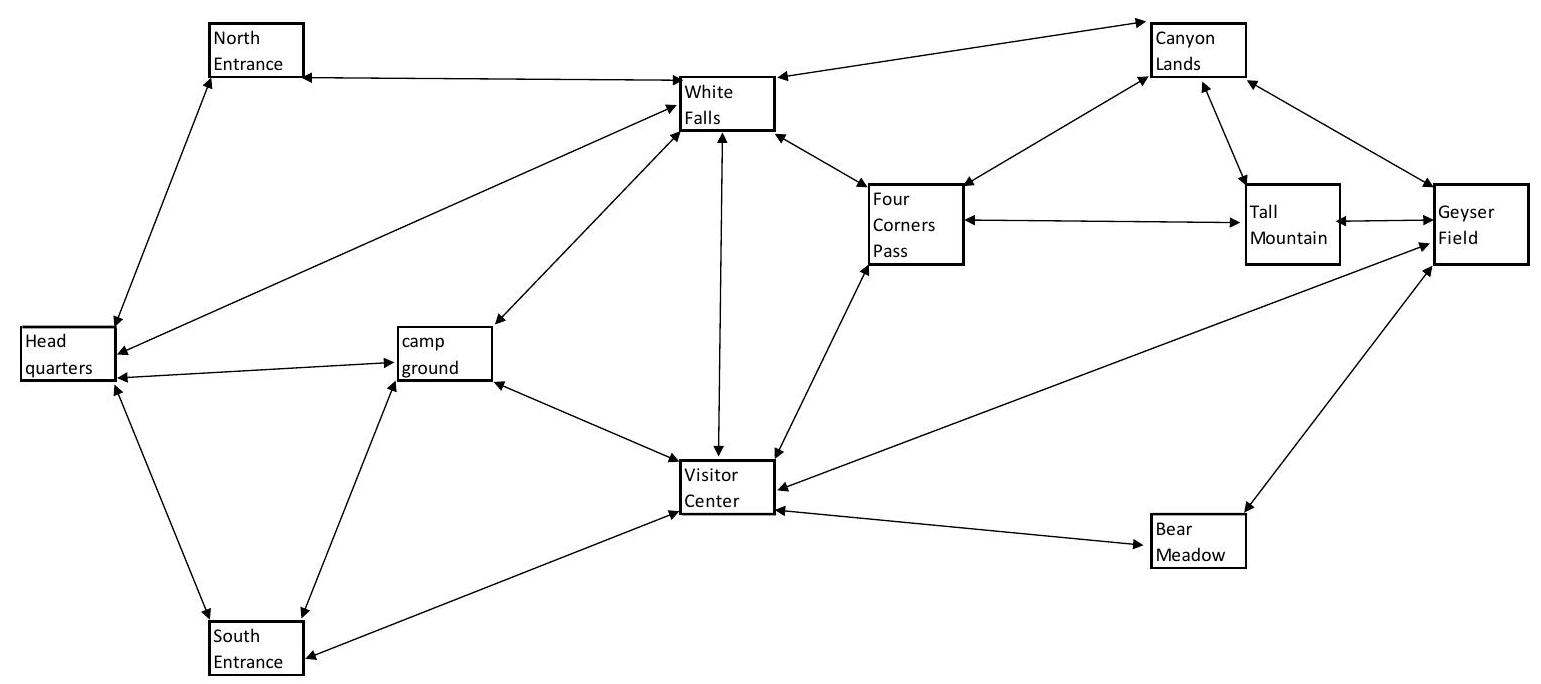
\includegraphics[width=\textwidth]{2024_12_09_1e11ad6a3005a73458cag-02}
\end{center}

\begin{resource}
For more information on real-world issues such as budget constraints and overcrowding in National Parks, see:
\begin{itemize}
\item \href{https://www.npca.org/articles/1500-budget-proposal-threatens-nationalparks}{https://www.npca.org/articles/1500-budget-proposal-threatens-nationalparks}
\item \href{http://www.ournationalparks.us/park}{http://www.ournationalparks.us/park} issues/busy parks seek approaches to manage crowds cars/ 
\item \href{https://www.nps.gov/zion/planyourvisit/traffic.htm}{https://www.nps.gov/zion/planyourvisit/traffic.htm}
\item \href{http://www.triplepundit.com/2016/03/national-parks-face-crowding-degradation/}{http://www.triplepundit.com/2016/03/national-parks-face-crowding-degradation/}
\item \href{http://www.hen.org/articles/arches-crowds-tourism-national-parks-utah}{http://www.hen.org/articles/arches-crowds-tourism-national-parks-utah}
\item \href{https://www.nps.gov/yell/planyourvisit/visitationstats.htm}{https://www.nps.gov/yell/planyourvisit/visitationstats.htm}
\end{itemize}
\end{resource}

\subsection{Allocation Problems: Resource Distribution}
Allocation problems involve distributing a limited resource (e.g., volunteer hours) from supply points (entrances and headquarters) to demand points (locations needing labor). The objective is often to minimize total cost.

This is an example of a classical transportation problem, a special case of linear programming. If total supply equals total demand, all resources are perfectly allocated. If not, we can introduce dummy variables (e.g., “excess” or “missing”) to handle imbalances.

\begin{example}{Volunteer Allocation}{volunteer-allocation}
Consider volunteer sources at HQ, NE, and SE, and destinations HQ, NE, SE, CG, VC, WF, CL, TM, BM, GF. Four corners pass does not need staffing and is omitted. This is a typical allocation problem: we have a resource (volunteer hours) to be distributed to various areas (park locations).

For instance, assume supply matches demand exactly:

\begin{center}
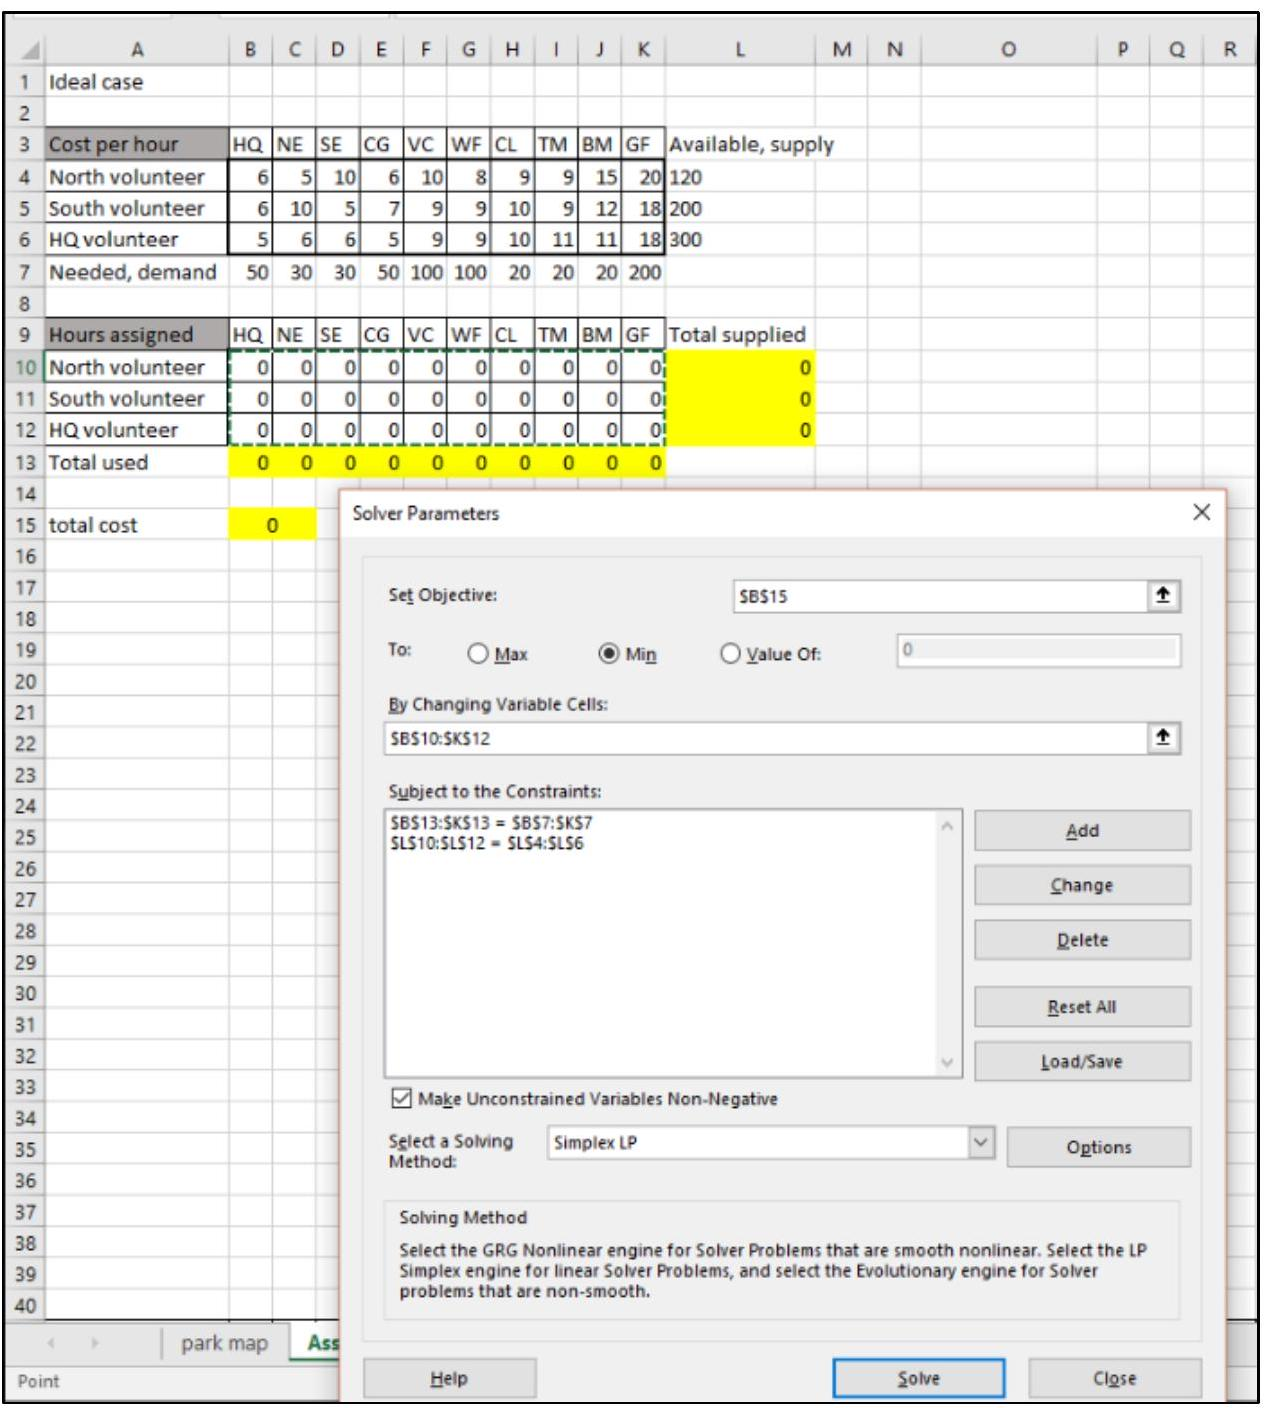
\includegraphics[width=1\textwidth]{2024_12_09_1e11ad6a3005a73458cag-03}
\end{center}

A linear program can be set up with the objective of minimizing total cost subject to the supply and demand constraints. Using a solver (e.g., Excel Solver), we obtain an optimal allocation of volunteers, for example at a total weekly cost of \$6,710. If supply exceeds demand, we add a dummy “excess” column; if supply is less than demand, we add a dummy “missing” row with prohibitively high cost, ensuring critical locations are served.
\end{example}

These refinements allow for flexible modeling of real-world conditions, such as too many or too few volunteers, or ensuring certain locations receive a minimum level of staffing.

\subsection{Assignment Problems: One-to-One Matching}
In assignment problems, we have a set of tasks and a set of agents (e.g., rangers) and must assign exactly one agent to each task. Unlike allocation, partial assignments are not allowed.

\begin{example}{Ranger Assignment}{ranger-assignment}
Suppose we must assign exactly one ranger to each location. We can model this as a standard assignment problem: the supply and demand for each task and agent is 1, and we solve for the minimal cost assignment. If a certain ranger cannot be assigned to a location, we give that pairing a very high cost, effectively ruling it out.

\begin{center}
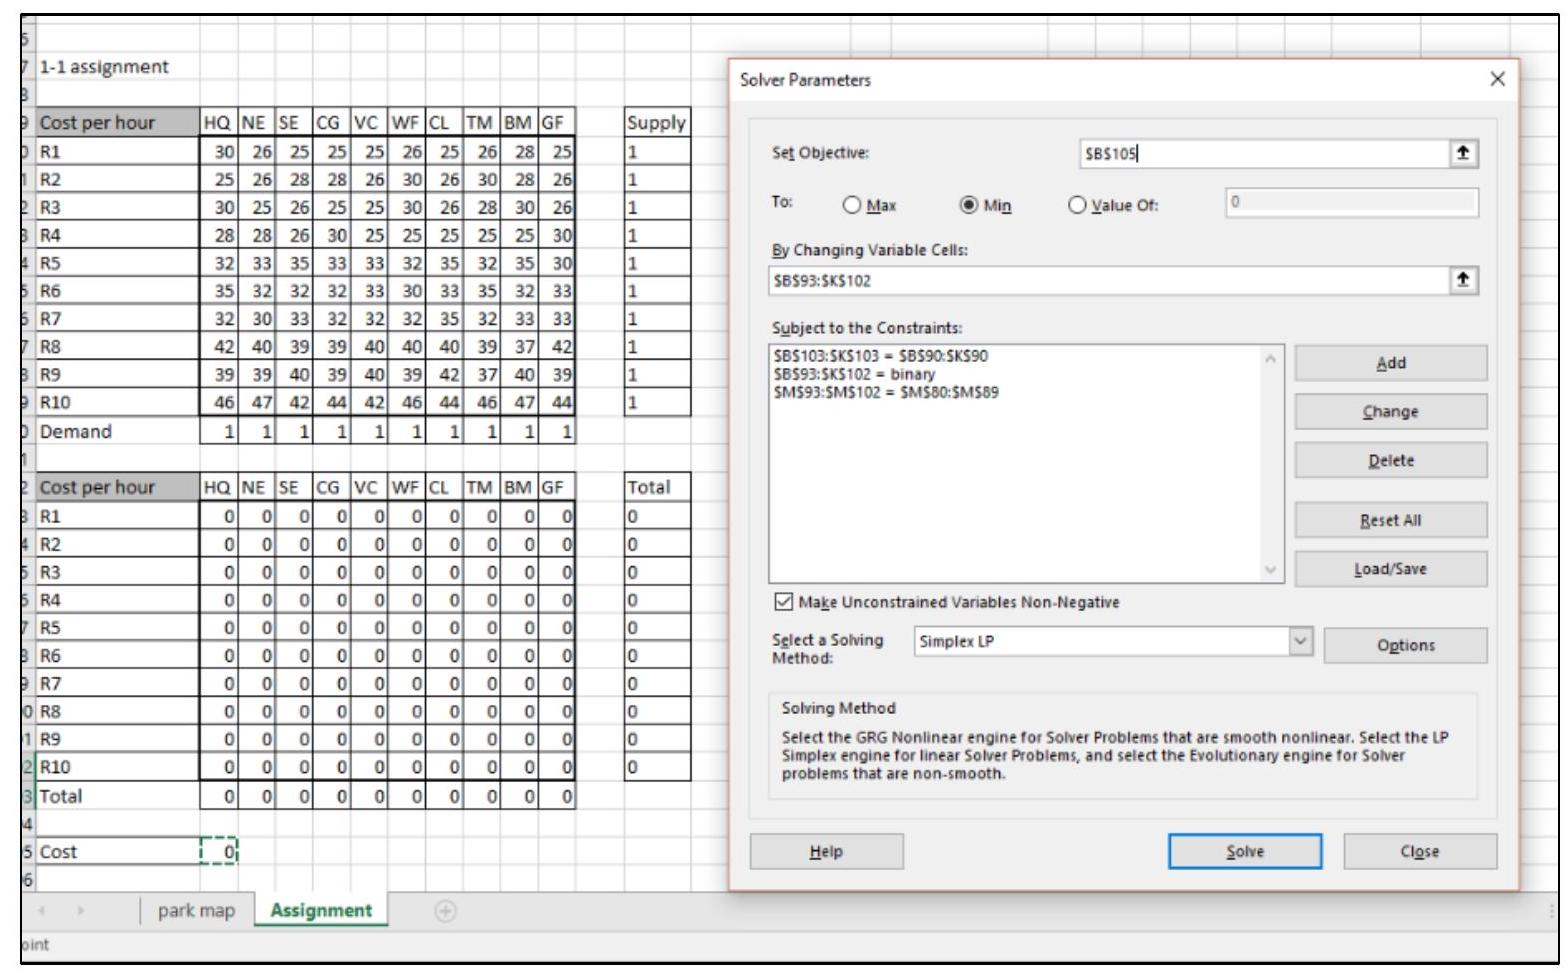
\includegraphics[width=0.7\textwidth]{2024_12_09_1e11ad6a3005a73458cag-06}
\end{center}

By solving this binary linear program or applying the Hungarian algorithm, we obtain a one-to-one assignment that minimizes total cost. The solver finds a feasible assignment with, for example, a total cost of \$306/hour.
\end{example}

\subsection{Network Problems}
Network models represent locations as nodes and roads as arcs. We consider several classical problems:

\begin{itemize}
  \item \textbf{Shortest Path:} Minimize the total cost (e.g., travel time) of a route from a start node (HQ) to an end node (GF).
  \item \textbf{Maximum Flow:} Maximize the amount of “flow” from a source (HQ) to a sink (GF) given arc capacities.
  \item \textbf{Minimum Spanning Tree (MST):} Minimize the total cost of connecting all nodes, useful for selecting roads to plow in winter.
  \item \textbf{Traveling Salesman Problem (TSP):} Find the shortest route visiting each node exactly once and returning to the start.
\end{itemize}

\subsubsection{Shortest Path Problem}
If we want the shortest route from HQ to GF, we can model each road segment as an arc with associated travel times.

\begin{center}
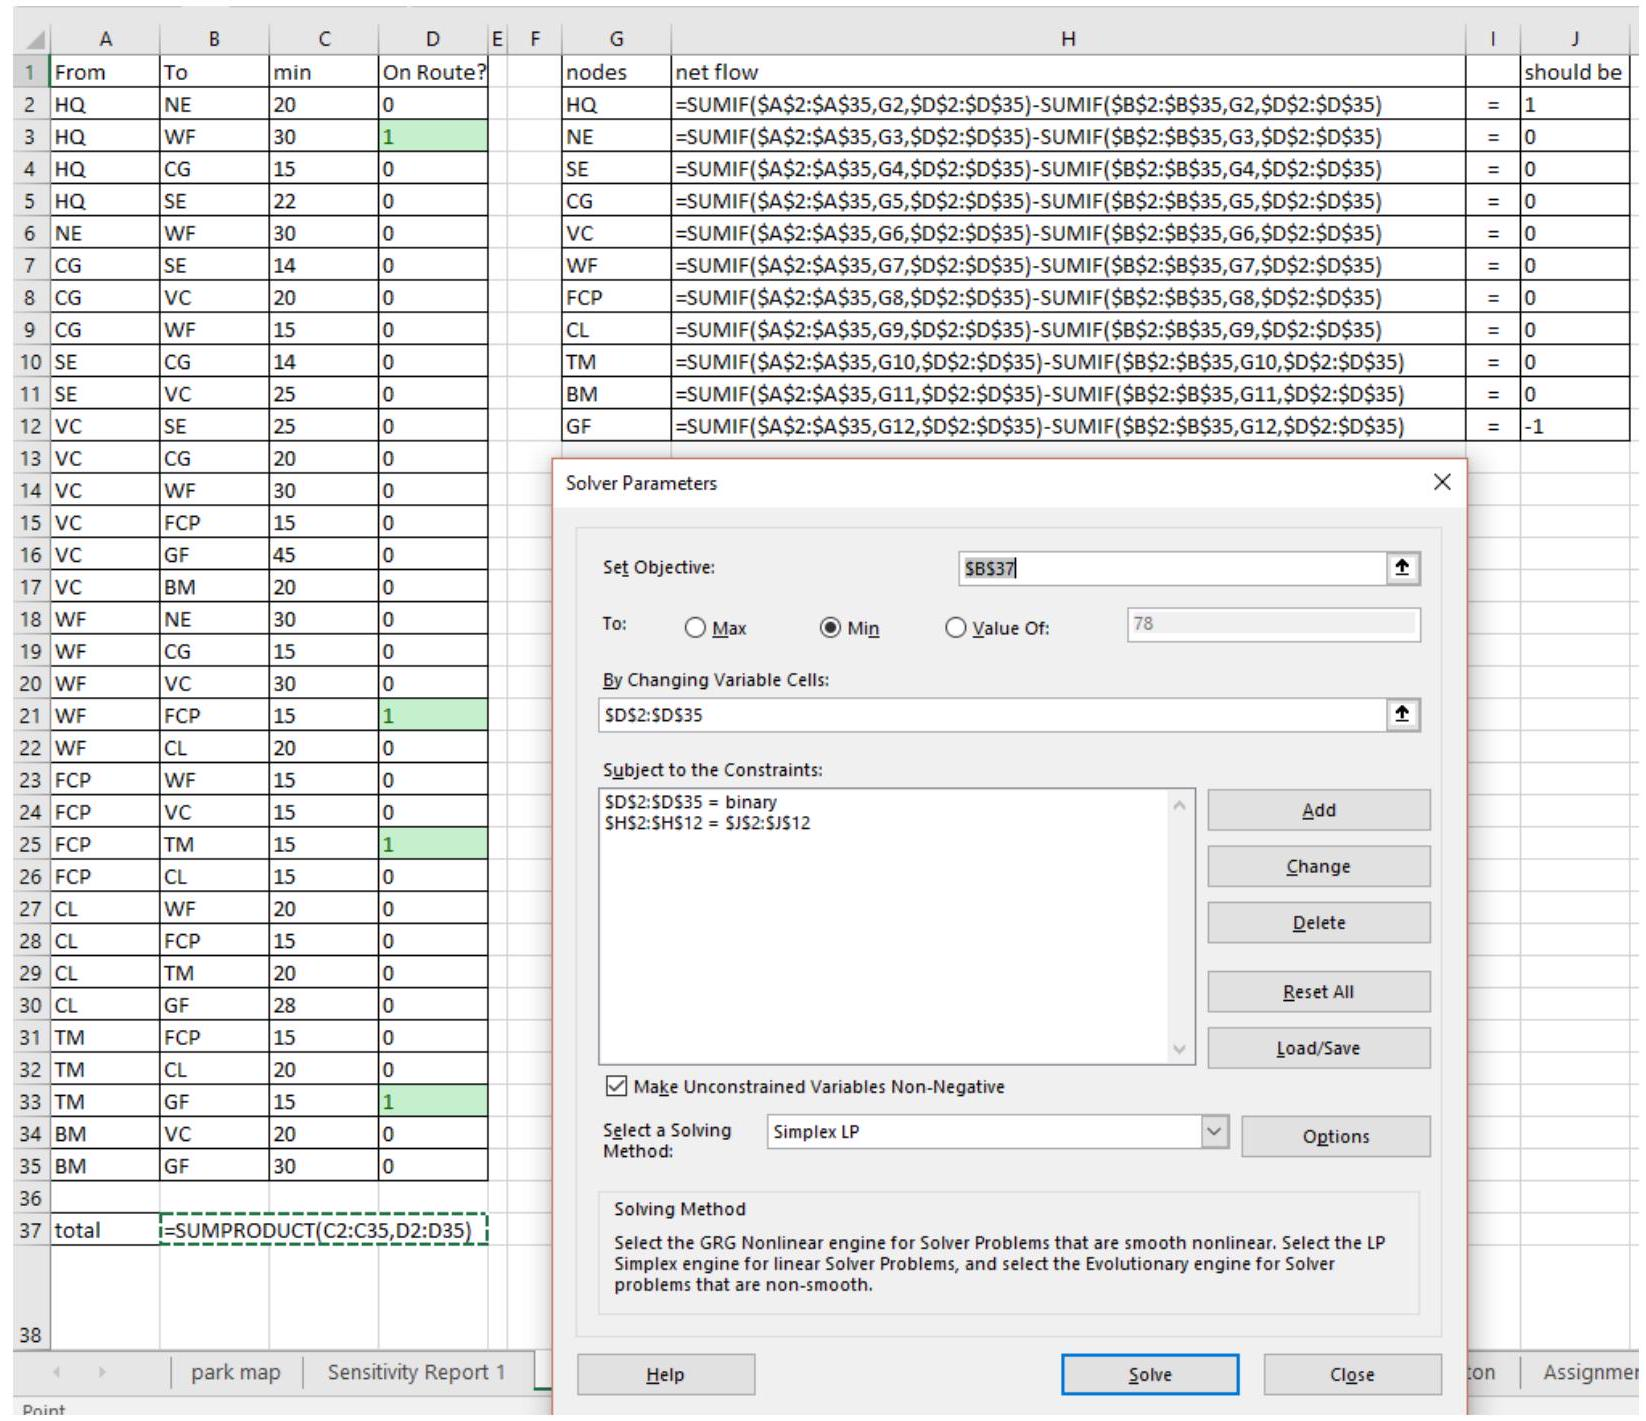
\includegraphics[width=0.5\textwidth]{2024_12_09_1e11ad6a3005a73458cag-09}
\end{center}

Using binary decision variables and net flow constraints, the solver yields a shortest path, for example: HQ $\rightarrow$ WF $\rightarrow$ FCP $\rightarrow$ TM $\rightarrow$ GF, with a total of 75 minutes.

\subsubsection{Maximum Flow and Minimum Cost Flow}
After identifying a single shortest path, we may want to send multiple shuttle buses. The maximum flow problem finds the greatest possible flow through the network. After determining maximum flow, a minimum cost flow formulation helps find the cheapest way to move that flow.

\begin{center}
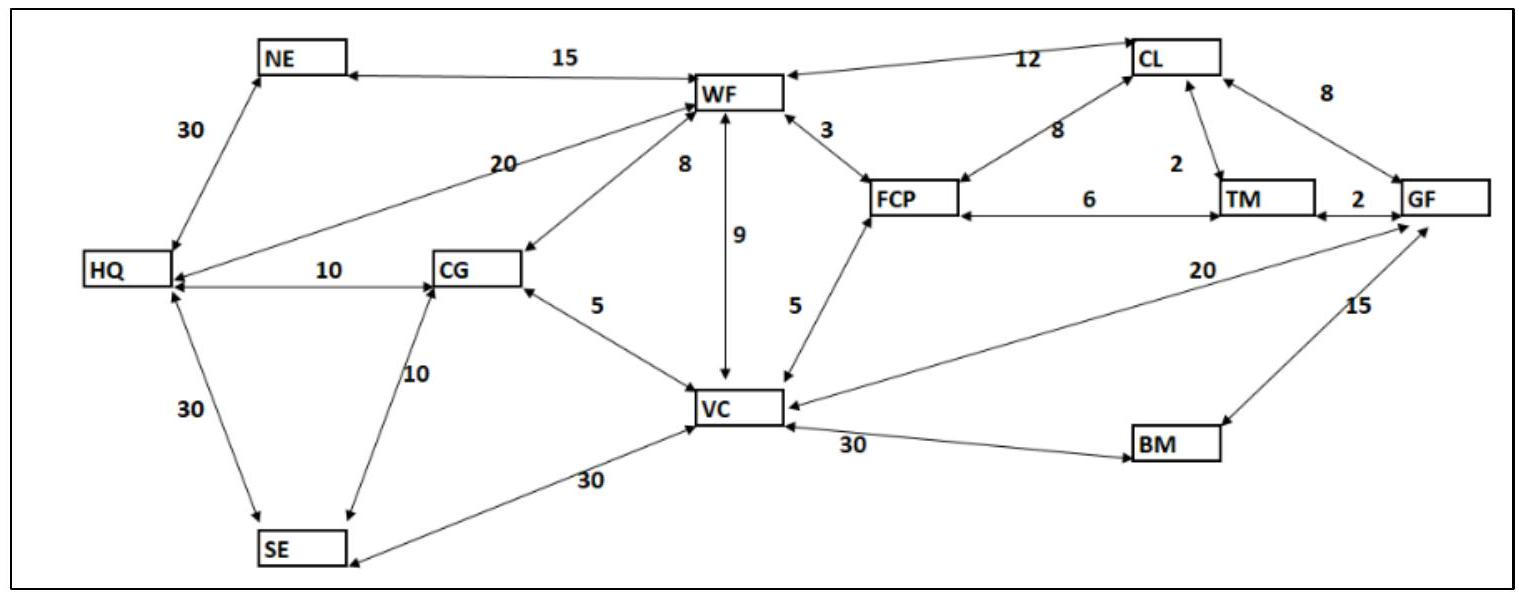
\includegraphics[width=0.8\textwidth]{2024_12_09_1e11ad6a3005a73458cag-10(2)}
\end{center}

By iteratively adjusting routes and capacities, we can find up to 45 shuttles per hour, each route chosen to minimize average travel time (around 90 minutes).

\subsection{Minimum Spanning Tree (MST)}
For winter plowing, we want all stations connected with minimal distance. This is a MST problem: pick the cheapest set of arcs that keeps the network connected without cycles.

\begin{center}
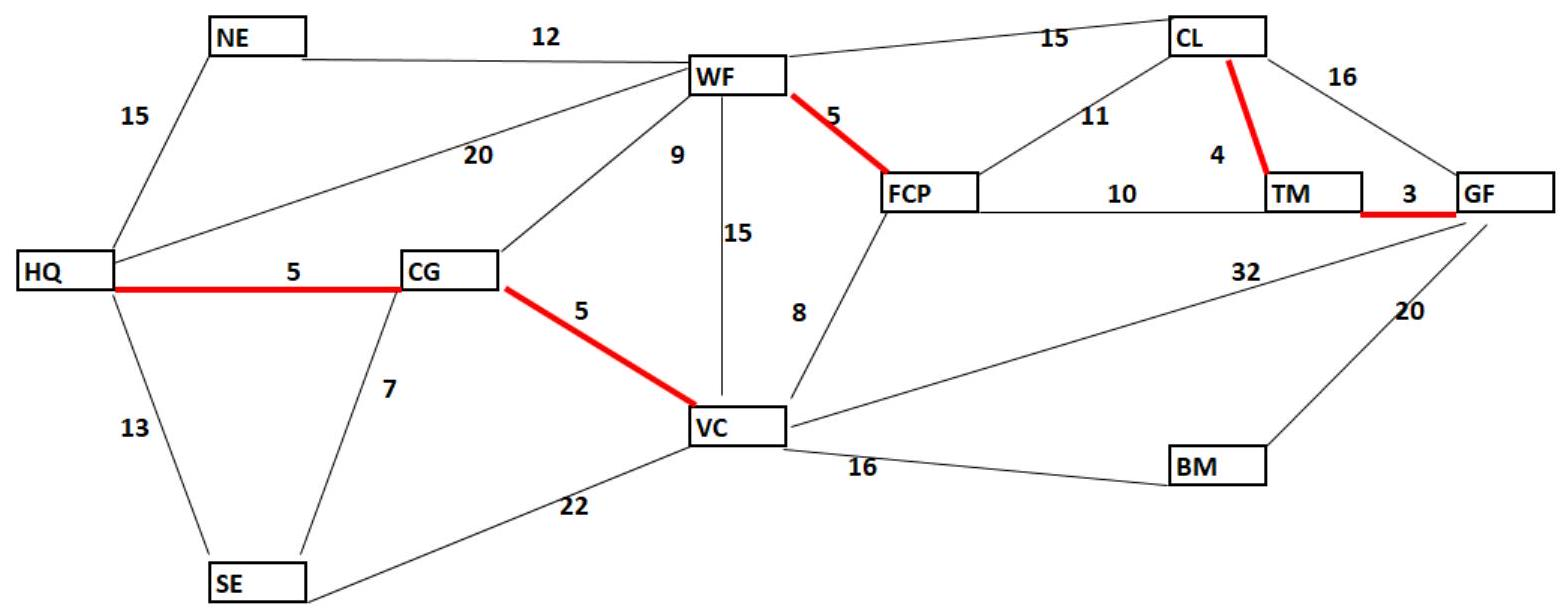
\includegraphics[width=0.5\textwidth]{2024_12_09_1e11ad6a3005a73458cag-13}
\end{center}

By greedily adding roads from shortest to longest while avoiding loops, we obtain a minimum spanning tree requiring 150 miles of plowing in total.

\subsection{Traveling Salesman Problem (TSP)}
In the TSP, we must visit every node exactly once and return to the start. With 11 locations, brute force checking of all permutations is infeasible. We apply heuristics such as the nearest neighbor approach, subtour reversal, or use Excel’s evolutionary solver.

\begin{example}{TSP Heuristic}{TSP}
Starting at HQ, using a nearest neighbor heuristic or a sub-tour reversal method, we find a circuit that visits all locations exactly once and returns to HQ.

\begin{center}
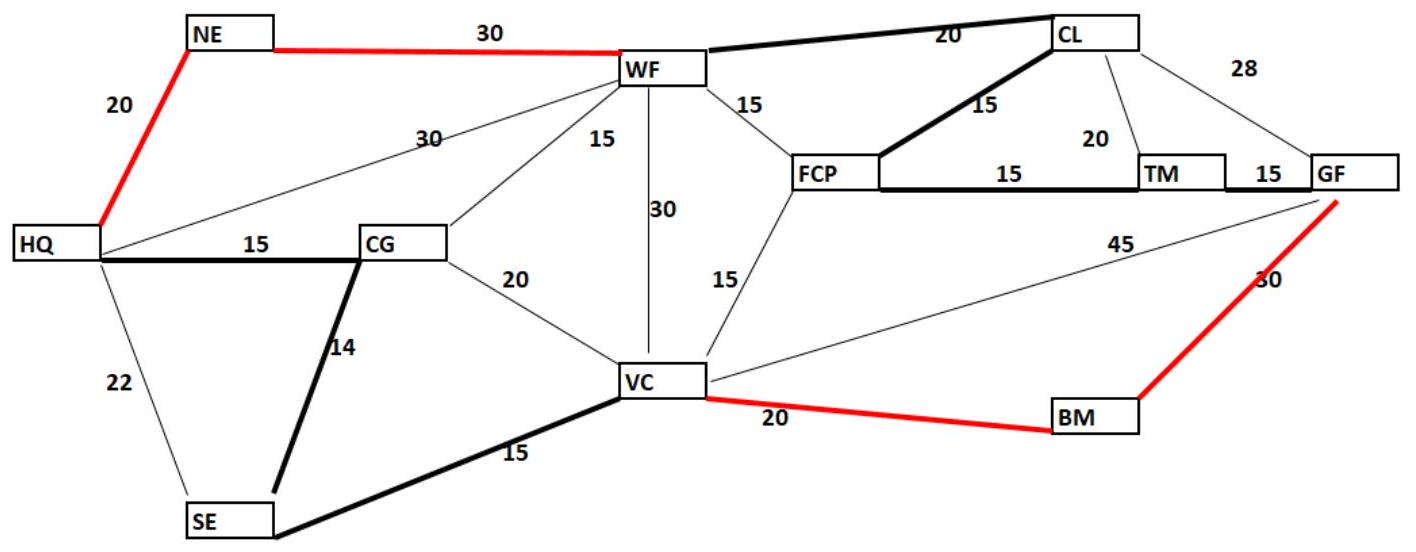
\includegraphics[width=0.8\textwidth]{2024_12_09_1e11ad6a3005a73458cag-16(2)}
\end{center}

The solution may not be provably optimal, but is often “good enough.” For instance, we can find a route that takes about 209 minutes total. Using the Excel evolutionary solver:

\begin{center}
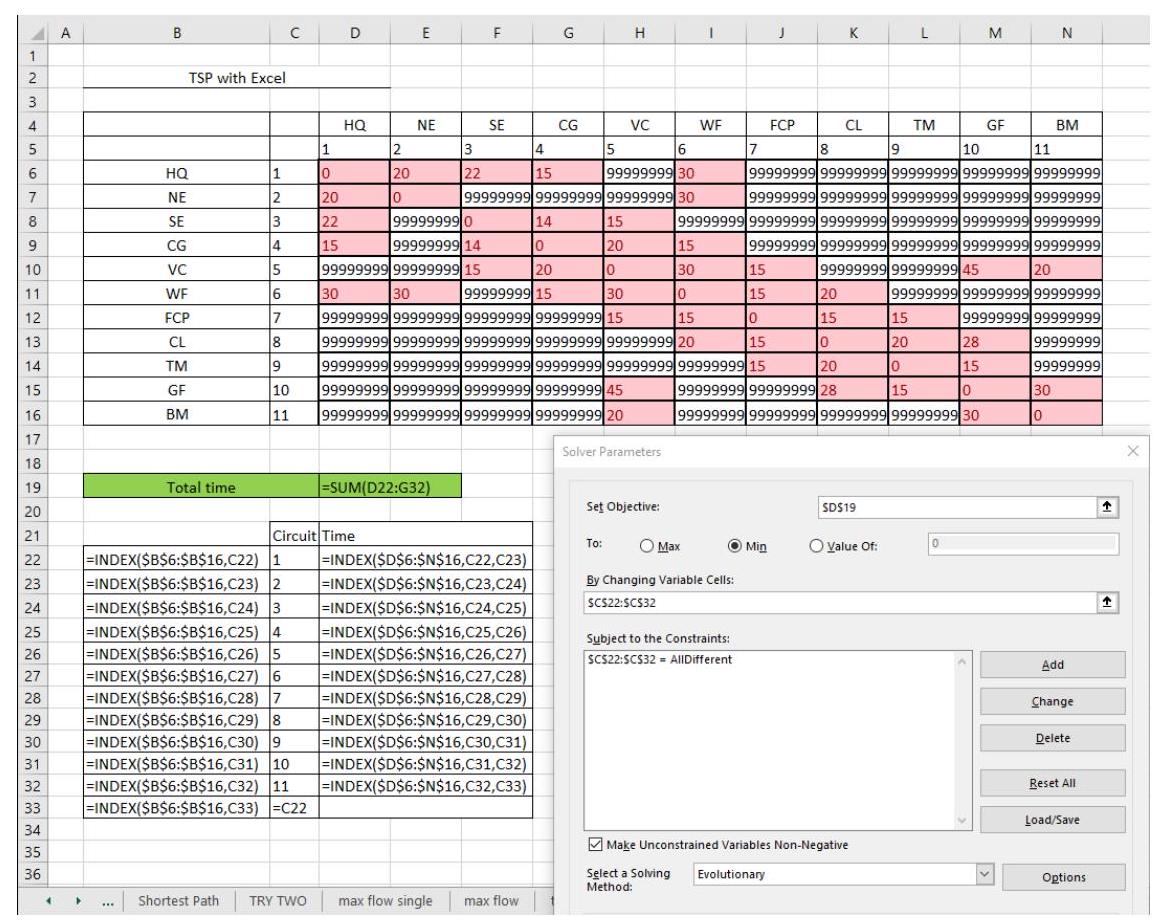
\includegraphics[width=0.6\textwidth]{2024_12_09_1e11ad6a3005a73458cag-19}
\end{center}

We obtain a route of similar total cost, confirming that the heuristic solution is reasonable.
\end{example}

\section{Road Patrols: Eulerian-Like Traversal}
For daily patrols covering all roads, we ideally want a Eulerian circuit (each edge used exactly once). If that is not possible (due to nodes having odd degree), we must repeat some roads.

\begin{center}
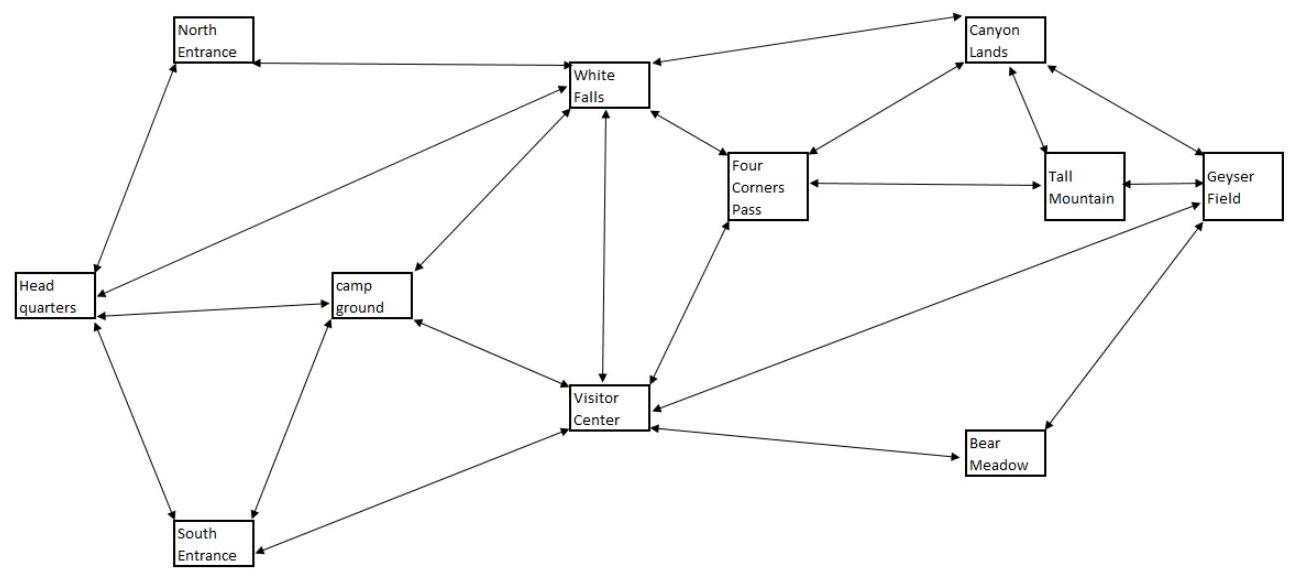
\includegraphics[width=0.8\textwidth]{2024_12_09_1e11ad6a3005a73458cag-20}
\end{center}

By setting up a linear/integer program ensuring each road is traveled at least once, we find a minimal-time route, for example 514 minutes (8 hours 34 minutes). While this may require some roads to be traversed multiple times, it ensures coverage at minimal cost.

\section{Conclusion and Further Considerations}
The examples in this chapter illustrate how classical optimization models—allocation, assignment, shortest path, MST, TSP, maximum flow, minimum cost flow, and Eulerian paths—can apply to practical scenarios in National Park management. By constructing these models and using computational tools, park managers can make informed, data-driven decisions.

Variations on these models allow incorporating more complex real-world constraints: supply shortages, minimum service levels, capacity expansions, or multi-objective considerations (e.g., balancing cost and environmental impact). Ultimately, these techniques provide a structured approach to solving complex problems, improving efficiency, and better serving both park visitors and ecosystem needs.





\chapter{Networks and Assignment in a National Park}
\todoChapter{{\color{gray}0\% complete. Goal: Update and format to match CC-BY-SA 4.0 license and previous style.}}
\begin{outcome}
\begin{itemize}
\item Understand how to formulate and solve allocation problems where supplies must meet demands.
\item Learn how to solve assignment problems, ensuring tasks are efficiently assigned to agents.
\item Explore network problems, including shortest path, maximum flow, minimum cost flow, and the traveling salesman problem.
\item Use spreadsheet tools (e.g., Excel) to model and solve these optimization problems.
\end{itemize}
\end{outcome}

\section{Introduction}
In this chapter, we consider a range of optimization problems that arise in a National Park setting. These problems include:

\begin{enumerate}
  \item \emph{Allocation Problems:} Distributing limited resources (such as volunteer hours) from supply points to various demand locations.
  \item \emph{Assignment Problems:} Matching agents (e.g., rangers) to tasks or locations in a one-to-one manner.
  \item \emph{Network Problems:} Finding shortest paths, spanning trees, maximum flows, and even tackling more complex routing challenges like the traveling salesman problem (TSP).
\end{enumerate}

We will illustrate how to model these problems as linear (and sometimes integer) programs and use common tools, such as Excel’s Solver, to find efficient solutions.

\section{Case Study: A National Park Under Pressure}
A popular National Park faces multiple challenges:

\begin{itemize}
  \item \textbf{Volunteer Assignment:} Due to budget cuts, many tasks like trail maintenance are done by volunteers. How can we assign volunteers and rangers to ensure each site is staffed efficiently?
  \item \textbf{Transportation Planning:} Traffic congestion may lead to banning personal vehicles and introducing shuttle buses. How do we design feasible shuttle routes and determine the necessary fleet size?
  \item \textbf{Winter Operations:} Some roads close in winter. Which roads must be plowed to ensure all ranger stations remain accessible with minimal cost?
  \item \textbf{Routing and Logistics:} A delivery truck must visit all park locations at least once. What is the most efficient route (a TSP-like problem)?
  \item \textbf{Daily Patrols:} Rangers must patrol all roads daily. What route minimizes total travel time, possibly traversing some roads multiple times if needed?
\end{itemize}

Below is a simplified park map showing roads and attractions. As needed, we will be given information on road length, travel time, and capacity. Throughout this chapter, we will refer to this map and the associated data tables.

\begin{center}
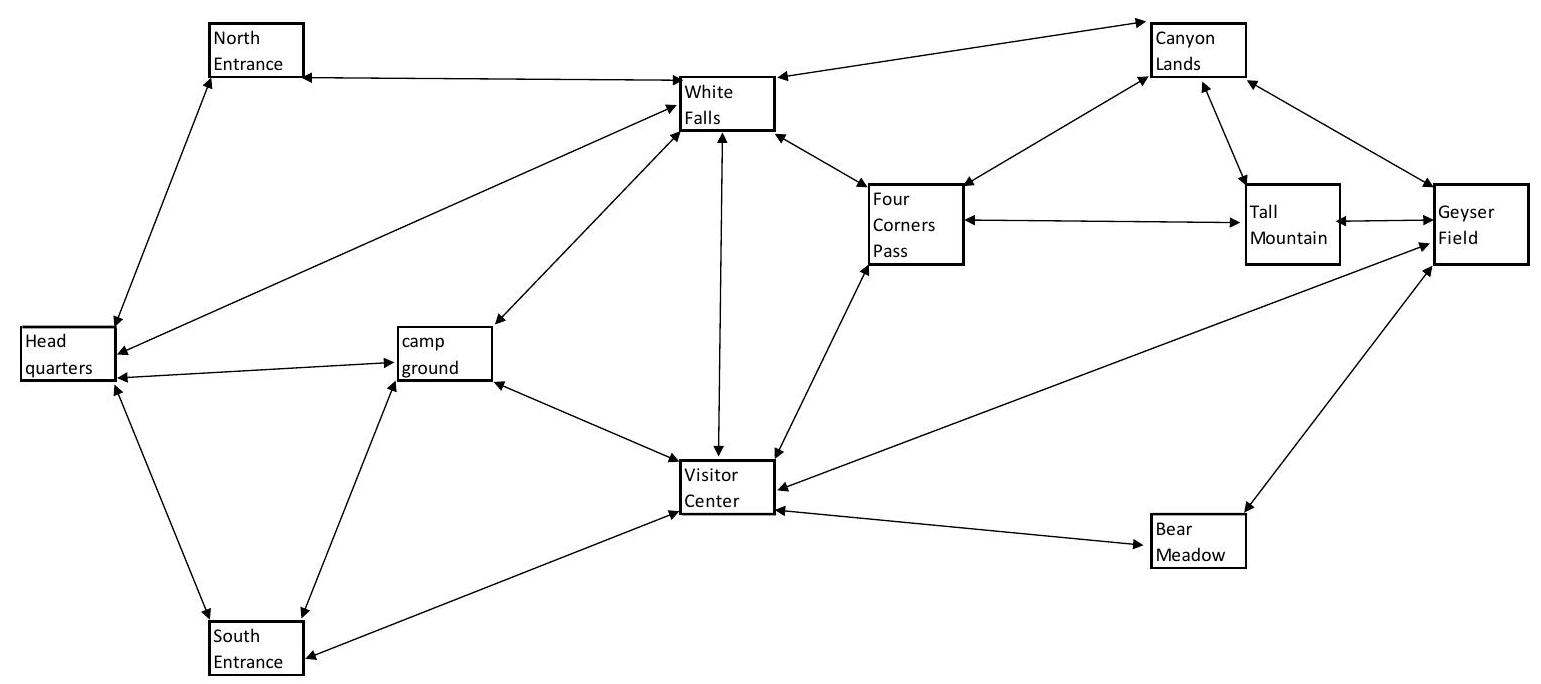
\includegraphics[width=0.5\textwidth]{2024_12_09_1e11ad6a3005a73458cag-02}
\end{center}

For more background on real-world issues facing National Parks, such as budget constraints and overcrowding, consult:

\begin{itemize}
  \item \href{https://www.npca.org/articles/1500-budget-proposal-threatens-nationalparks}{https://www.npca.org/articles/1500-budget-proposal-threatens-nationalparks}
  \item \href{https://www.nps.gov/zion/planyourvisit/traffic.htm}{https://www.nps.gov/zion/planyourvisit/traffic.htm}
  \item \href{https://www.triplepundit.com/2016/03/national-parks-face-crowding-degradation/}{https://www.triplepundit.com/2016/03/national-parks-face-crowding-degradation/}
\end{itemize}

\section{Allocation Problems: Resource Distribution}
Allocation problems involve distributing a limited resource (e.g., volunteer hours) from supply points (entrances and headquarters) to demand points (locations needing labor). The objective is often to minimize total cost.

\subsection*{Example: Volunteer Allocation}
Consider a situation where volunteers are available at certain park entrances and must be allocated to various locations. The cost per volunteer hour differs by source-location pair. We assume, initially, that total supply matches total demand exactly.

\begin{example}{Volunteer Allocation}{allocation}
We have three volunteer sources (North, South, and HQ) and multiple demand locations (HQ, NE, SE, CG, VC, WF, CL, TM, BM, GF). The table below gives the cost per volunteer hour and the supply and demand at each location:

\begin{center}
\begin{tabular}{|c|c|c|c|c|c|c|c|c|c|c|c|}
\hline
Cost/hr & HQ & NE & SE & CG & VC & WF & CL & TM & BM & GF & Supply \\
\hline
North & 6 & 5 & 10 & 6 & 10 & 8 & 9 & 9 & 15 & 20 & 120 \\
\hline
South & 6 & 10 & 5 & 7 & 9 & 9 & 10 & 9 & 12 & 18 & 200 \\
\hline
HQ & 5 & 6 & 6 & 5 & 9 & 9 & 10 & 11 & 11 & 18 & 300 \\
\hline
Demand & 50 & 30 & 30 & 50 &100 &100 & 20 & 20 & 20 & 200 &  \\
\hline
\end{tabular}
\end{center}

Total supply equals total demand (620), so all volunteer hours can be perfectly allocated. Using linear programming (with the objective of minimizing total cost subject to supply and demand constraints), we can solve this problem. Setting this up in a spreadsheet solver yields an optimal solution with a total cost of \$6,710 per hour.
\end{example}

\subsection*{Adjusting Supply and Demand}
If supply exceeds demand, we introduce a dummy “excess” category to absorb unused volunteer hours at zero cost. If supply is less than demand, we can introduce a “missing volunteers” category with a prohibitively high cost to ensure demand is met where most critical. Adjusting the cost structure and constraints allows us to model more complex scenarios, such as mandatory staffing levels at certain locations or flexible minimum/maximum requirements.

\section{Assignment Problems: One-to-One Matching}
In assignment problems, we have a set of tasks and a set of agents (e.g., rangers) and we must assign each agent exactly one task (and vice versa) to minimize cost or maximize efficiency. Unlike allocation problems, the resources cannot be fractionally divided; each agent must be assigned to exactly one task.

\begin{example}{Ranger Assignment}{assignment}
Suppose we have 10 locations needing exactly one full-time ranger each, and 10 rangers available. If a ranger cannot work a certain location, we assign a large cost to that pairing, ensuring it is never chosen. By solving the assignment problem (using a standard linear programming approach with binary variables or the Hungarian algorithm), we obtain the one-to-one assignments at minimal cost.
\end{example}

\section{Network Problems}
Network models involve nodes (locations) and arcs (roads). Common questions include:

\begin{itemize}
  \item \textbf{Shortest Path:} Find the least-cost route from a start to an end node.
  \item \textbf{Maximum Flow:} Determine the greatest amount of flow that can move through a network from a source to a sink.
  \item \textbf{Minimum Spanning Tree:} Connect all nodes with the minimum total arc cost.
  \item \textbf{Traveling Salesman Problem (TSP):} Find the shortest route visiting each node exactly once and returning to the start.
\end{itemize}

\subsection{Shortest Path Problem}
If we want the shortest time route from HQ to GF, we can model each road segment as an arc with a travel time. Using binary decision variables to indicate if a segment is chosen, and net flow constraints (1 for HQ as a source, -1 for GF as a sink, and 0 for intermediate nodes), we can ensure that a chosen set of arcs forms a continuous path. Running a solver yields the shortest path and total travel time.

\subsection{Maximum Flow and Minimum Cost Flow}
After finding a single shortest path, we may want to push as many shuttle buses as possible from HQ to GF, subject to capacity constraints on each road. This leads to a maximum flow problem. Once we know the maximum flow, we can introduce costs (e.g., travel time or expense) to find a minimum cost flow solution that achieves a desired flow level at minimal cost.

\subsection{Minimum Spanning Tree (MST)}
For the winter plowing problem, we want to ensure all locations remain accessible at minimal cost. This is equivalent to finding a minimum spanning tree (MST): a subset of roads that connects all points with the least total mileage. By using a greedy algorithm (e.g., Kruskal’s or Prim’s method), we identify which roads should remain open and plowed, thereby minimizing total plowing mileage.

\subsection{Traveling Salesman Problem (TSP)}
The TSP requires finding the shortest tour visiting all locations exactly once and returning to the start. This is computationally challenging. We rely on heuristics (e.g., nearest neighbor) and improvement algorithms (e.g., subtour reversal) or rely on a solver’s built-in heuristics (e.g., Excel’s evolutionary solver) to find a good, if not provably optimal, solution.

\begin{example}{TSP Heuristic}{TSP}
Consider needing to deliver supplies to each of the 11 locations in a single loop starting and ending at HQ. The brute force approach is infeasible due to the enormous number of possible tours. Instead, we try a nearest neighbor heuristic or subtour reversal to quickly find a “good” route. While not guaranteed optimal, these heuristics often yield routes that are short and practical.
\end{example}

\section{Road Patrols: Eulerian-Like Traversal}
For daily patrols, we must traverse every road at least once, starting and ending at HQ. Ideally, this would form an Eulerian circuit (each edge visited exactly once). If that is not possible (because not all nodes have even degree), we must repeat some roads. Using a linear programming approach with integer constraints to ensure each road is covered at least once, we find a feasible route that minimizes total travel time. While this might require driving some roads multiple times, it ensures comprehensive coverage.

\section{Conclusion and Further Considerations}
The scenarios presented illustrate how classical optimization models—allocation, assignment, network flows, shortest paths, MSTs, TSPs, and Eulerian tours—can apply to real-world problems in a National Park context. By constructing these models and using common computational tools, park managers can make informed decisions. Moreover, variations on these models allow for practical considerations such as supply shortages, extra capacity, enforced minimum service levels, and more.

Ultimately, these modeling techniques offer a systematic way to balance cost, efficiency, and accessibility when managing complex systems like National Parks.




==================

\chapter*{Original}
\section*{NATIONAL PARK - NETWORKS AND ASSIGNMENT}
In this chapter, we will examine three types of problems:

\begin{enumerate}
  \item In allocation problems, a limited resource "supply" is allocated to various entities "demand". We will see what happens if demand exceeds supply and vice versa.
  \item Assignment problems assign exactly one of $n$ task to each of exactly $n$ workers
  \item Network problems look at a variety of issues arising in a network of nodes and arcs, from spanning trees to traversal problems.
\end{enumerate}

\section*{Learning Goals}
\begin{itemize}
  \item Allocation problems
  \item Assignment problems
  \item Shortest path problem
  \item Flow problems
  \item Maximum flow
  \item Maximum flow - minimum cost
  \item Traveling salesman problem
  \item Using Excel to solve the above
\end{itemize}

\section*{Case Study Description}
A very popular National Park is facing a number of challenges and has hired your company to propose solutions to the following:

\begin{enumerate}
  \item Due to budget cuts, much of the work in the park such as interpretive services and trail maintenance is done by volunteers. What is the most efficient way to assign them to the various tasks and locations? Also, you need to make sure each location has one full-time ranger on site.
  \item Traffic has gotten so bad that the park is considering banning personal vehicles on some roads and using shuttle busses instead. What should the bus routes be? How many busses are needed? Is a shuttle service even feasible?
  \item During winter, some of the park roads will be closed. However, enough roads need to be plowed to allow access to all ranger stations. Which roads should be plowed?
  \item A delivery truck needs to visit each of the parks location. What is the best route to take?
  \item All roads need to be patrolled daily. What is the best route for the ranger to take?
\end{enumerate}

Following is a simplified park map showing roads and attractions. As needed, you will also be provided with information regarding length, driving time, and shuttle capacity for each road segment.\\

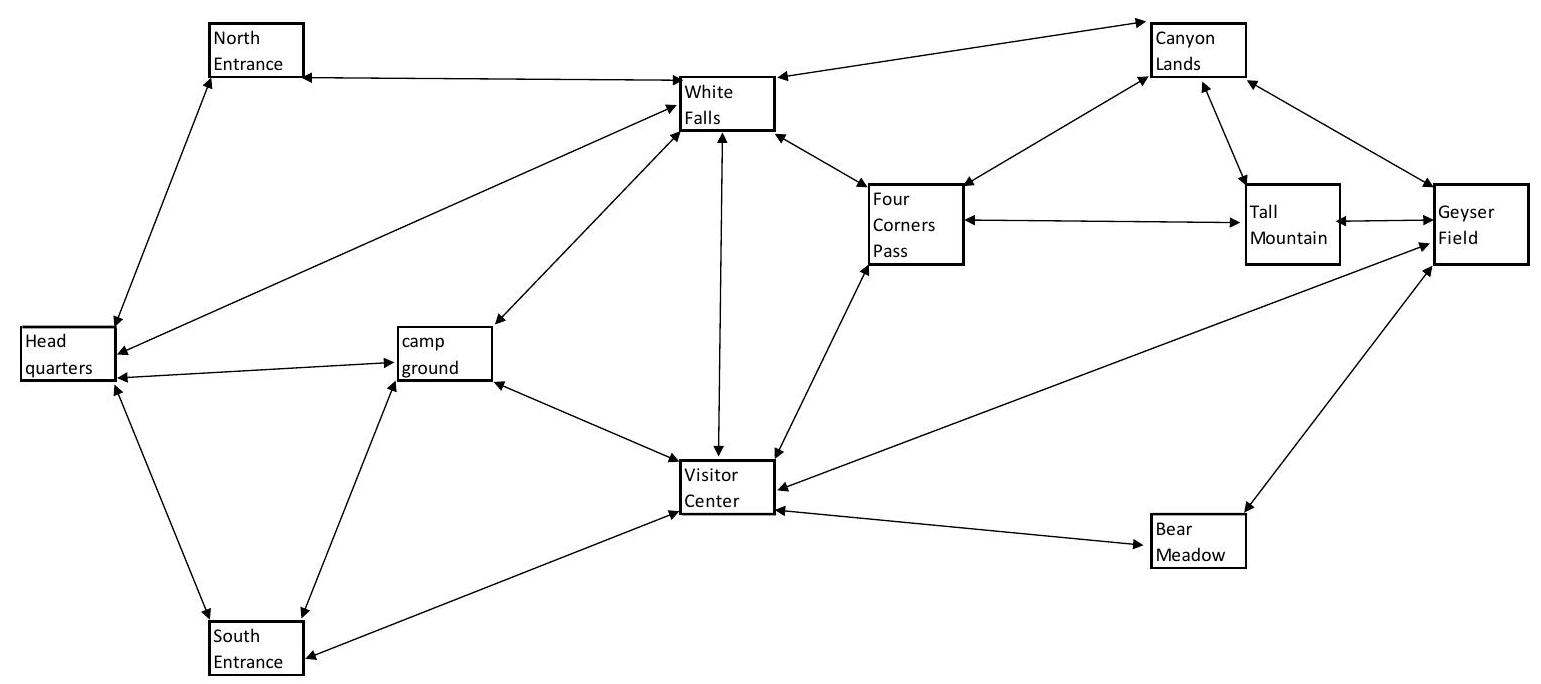
\includegraphics[width=0.95\textwidth]{2024_12_09_1e11ad6a3005a73458cag-02}

\section*{References}
Budget cuts and overcrowding are very real issues for our National Parks. For more information on both, see:\\
\href{https://www.npca.org/articles/1500-budget-proposal-threatens-nationalparks#sm.0000ks3wtu35mdezurz1liyktck1t}{https://www.npca.org/articles/1500-budget-proposal-threatens-nationalparks\#sm.0000ks3wtu35mdezurz1liyktck1t}\\
\href{http://www.ournationalparks.us/park}{http://www.ournationalparks.us/park} issues/busy parks seek approaches to manag e crowds cars/ \href{https://www.nps.gov/zion/planyourvisit/traffic.htm}{https://www.nps.gov/zion/planyourvisit/traffic.htm}\\
\href{http://www.triplepundit.com/2016/03/national-parks-face-crowding-degradation/}{http://www.triplepundit.com/2016/03/national-parks-face-crowding-degradation/} \href{http://www.hen.org/articles/arches-crowds-tourism-national-parks-utah}{http://www.hen.org/articles/arches-crowds-tourism-national-parks-utah} \href{https://www.nps.gov/yell/planyourvisit/visitationstats.htm}{https://www.nps.gov/yell/planyourvisit/visitationstats.htm}

\section*{Part 1: Work Force - Resource Allocation}
Let's assume volunteers are available at the entrances to the park, $\mathrm{HQ}, \mathrm{NE}$, and SE . From there, you will have to transport them to the different locations and tasks. There is trail construction going on at VC and GF, so a lot of volunteers are needed there. GF is a very popular tourist destination, so lots of help is needed there as well. The cost/volunteer hour depends on a number of factors, such as distance to park entrance, nature of work, insurances required, etc. This table shows a summary of cost, supply, and demand.\\
We will denote each location by its initials, for example NE for North entrance, CL for Canyon lands etc. Four corners pass does not need any staffing, so we omit it.\\
This is an example of an allocation problem. A resource (volunteer hours, water rights, money, fish catch) is allocated to different areas (park location, cities, departments, canneries). In the ideal case, supply matches demand exactly. Let's start by assuming this is happening here:

\begin{center}
\begin{tabular}{|c|c|c|c|c|c|c|c|c|c|c|c|}
\hline
Cost per hour & HQ & NE & SE & CG & VC & WF & CL & TM & BM & GF & Supply \\
\hline
North volunteer & 6 & 5 & 10 & 6 & 10 & 8 & 9 & 9 & 15 & 20 & 120 \\
\hline
South volunteer & 6 & 10 & 5 & 7 & 9 & 9 & 10 & 9 & 12 & 18 & 200 \\
\hline
HQ volunteer & 5 & 6 & 6 & 5 & 9 & 9 & 10 & 11 & 11 & 18 & 300 \\
\hline
Demand & 50 & 30 & 30 & 50 & 100 & 100 & 20 & 20 & 20 & 200 &  \\
\hline
\end{tabular}
\end{center}

Note how the supply column and demand row add up to the same value, 620. Your objective is to minimize cost while meeting demand. Note that in this ideal case supply = demand. This problem can be set up as a linear programming problem and solved with the simplex method. You should check that the assumptions for a LP problem hold.\\
To solve this problem with Excel, we set up a second table containing the decision variables, i.e. how many hours from which source are being allocated to which area. Initially, we set them all to zero. The highlighted cells contain formulas. We can now use the Excel solver.\\
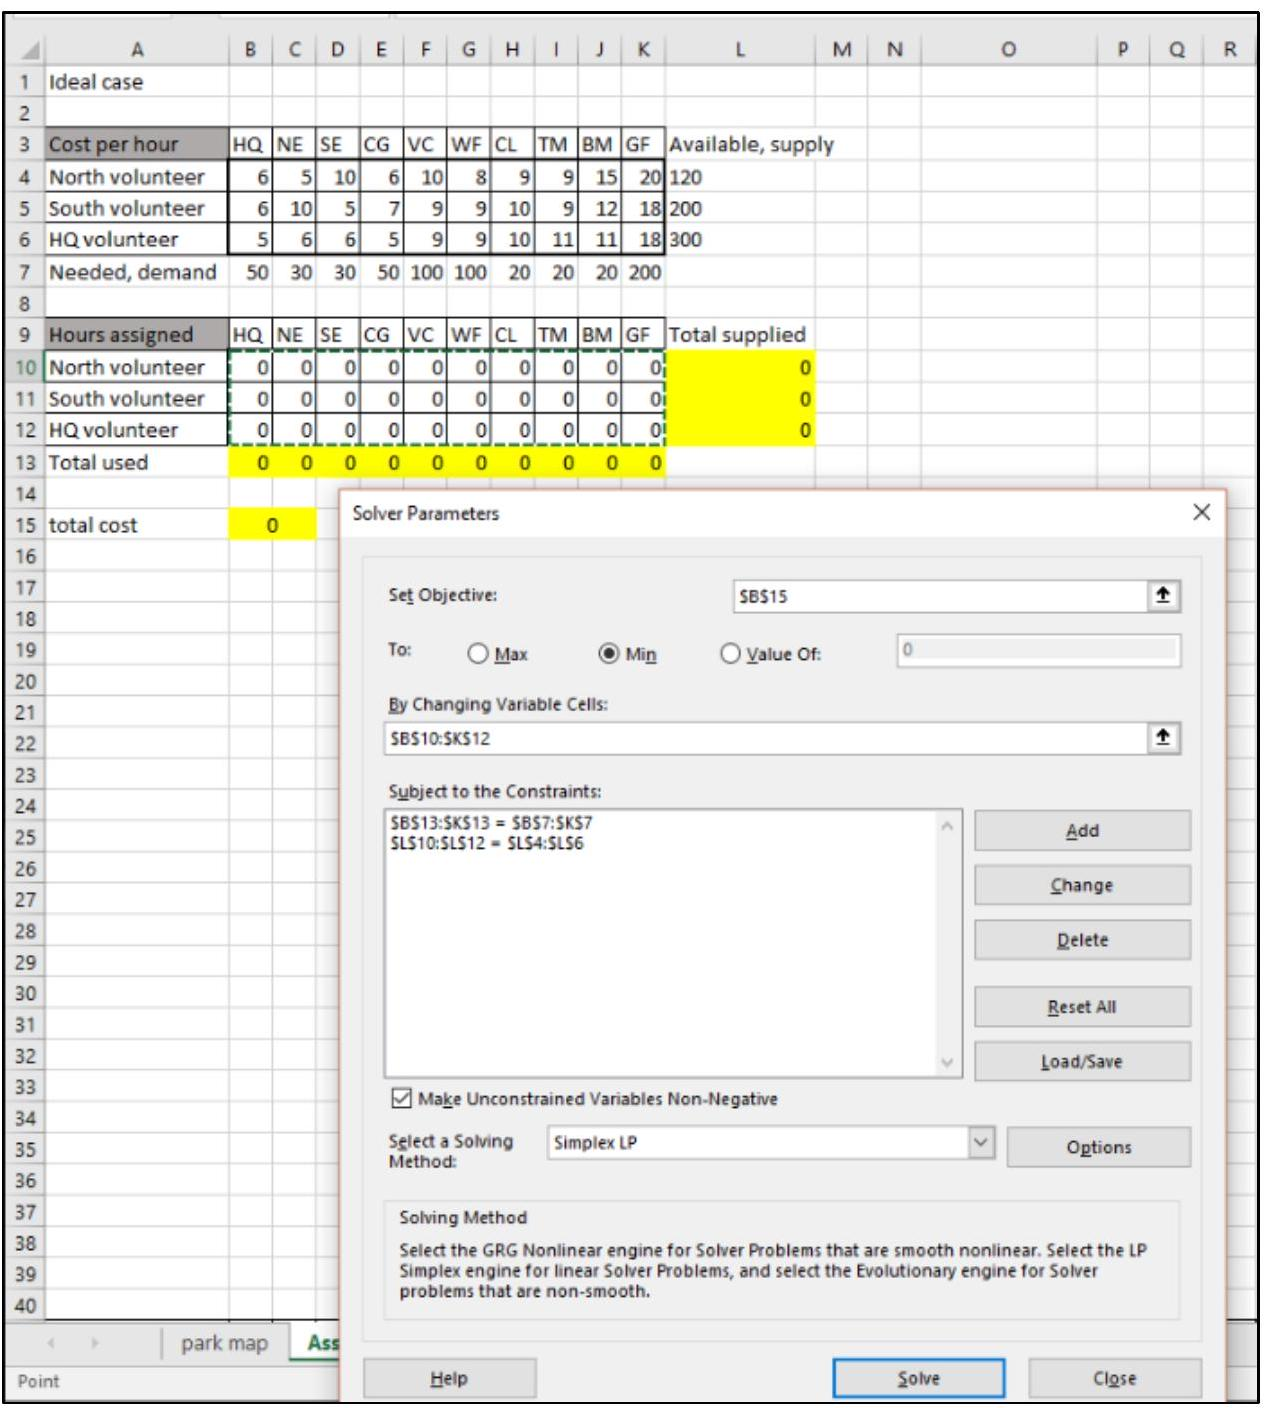
\includegraphics[width=0.5\textwidth]{2024_12_09_1e11ad6a3005a73458cag-03}

The solver returns the solution, which the park can then implement, and the total weekly cost of $\$ 6710$.

\begin{center}
\begin{tabular}{|l|r|r|r|r|r|r|r|r|r|r|l|}
\hline
Hours assigned & HQ & NE & SE & CG & VC & WF & CL & TM & BM & GF & Total supplied \\
\hline
North volunteer & 0 & 0 & 0 & 0 & 0 & 100 & 20 & 0 & 0 & 0 & 120 \\
\hline
South volunteer & 0 & 0 & 30 & 0 & 0 & 0 & 0 & 20 & 0 & 150 & 200 \\
\hline
HQ volunteer & 50 & 30 & 0 & 50 & 100 & 0 & 0 & 0 & 20 & 50 & 300 \\
\hline
Total used & 50 & 30 & 30 & 50 & 100 & 100 & 20 & 20 & 20 & 200 &  \\
\hline
total cost & 6710 & \multicolumn{4}{|c|}{} &  &  &  &  &  &  \\
\hline
\end{tabular}
\end{center}

We were lucky and got integer value solutions. However, in this case the divisibility requirement of LP problems is satisfied, we could allow fractional hours worked.

\section*{Refinements}
Let's assume you have too many volunteers, i.e. supply > demand. We incorporate them by assigning those hours we don't need to the "excess" column and proceeding otherwise just like before:

\begin{center}
\begin{tabular}{|l|r|r|r|r|r|r|r|r|r|r|r|}
\hline
Cost per hour & \multicolumn{1}{l|}{HQ} & NE & \multicolumn{1}{l|}{SE} & CG & VC & WF & CL & TM & BM & GF & excess \\
\hline
North volunteer & 6 & 5 & 10 & 6 & 10 & 8 & 9 & 9 & 15 & 20 & 0 \\
\hline
South volunteer & 6 & 10 & 5 & 7 & 9 & 9 & 10 & 9 & 12 & 18 & 0 \\
\hline
HQ volunteer & 5 & 6 & 6 & 5 & 9 & 9 & 10 & 11 & 11 & 18 & 0 \\
\hline
Demand & 50 & 30 & 30 & 50 & 100 & 100 & 20 & 20 & 20 & 200 & 130 \\
\hline
\end{tabular}
\end{center}

\begin{center}
\begin{tabular}{|l|}
\hline
supply \\
\hline
200 \\
\hline
250 \\
\hline
300 \\
\hline
\end{tabular}
\end{center}

\begin{center}
\begin{tabular}{|l|r|r|r|r|r|r|r|r|r|r|r|}
\hline
Hours assigned & \multicolumn{1}{l|}{HQ} & NE & \multicolumn{1}{l|}{SE} & \multicolumn{1}{l|}{CG} & VC & WF & CL & TM & BM & GF & excess \\
\hline
North volunteer & 0 & 0 & 0 & 0 & 0 & 0 & 0 & 0 & 0 & 0 & 0 \\
\hline
South volunteer & 0 & 0 & 0 & 0 & 0 & 0 & 0 & 0 & 0 & 0 & 0 \\
\hline
HQ volunteer & 0 & 0 & 0 & 0 & 0 & 0 & 0 & 0 & 0 & 0 & 0 \\
\hline
Total used & 0 & 0 & 0 & 0 & 0 & 0 & 0 & 0 & 0 & 0 & 0 \\
\hline
\end{tabular}
\end{center}

\begin{center}
\begin{tabular}{|r|}
\hline
\begin{tabular}{l}
Total \\
supplied \\
\end{tabular} \\
\hline
0 \\
\hline
0 \\
\hline
0 \\
\hline
\end{tabular}
\end{center}

\begin{verbatim}
total cost \
\end{verbatim}

The table below shows the solution. Not surprisingly, with more volunteers available the overall cost went down.

\begin{center}
\begin{tabular}{|l|c|c|c|c|c|c|c|c|c|c|c|}
\hline
Hours assigned & HQ & NE & SE & CG & VC & WF & CL & TM & BM & GF & not used \\
\hline
North volunteer & 0 & 30 & 0 & 0 & 0 & 100 & 20 & 20 & 0 & 0 & 30 \\
\hline
South volunteer & 0 & 0 & 30 & 0 & 100 & 0 & 0 & 0 & 0 & 20 & 100 \\
\hline
HQ volunteer & 50 & 0 & 0 & 50 & 0 & 0 & 0 & 0 & 20 & 180 & 0 \\
\hline
\end{tabular}
\end{center}

\begin{center}
\begin{tabular}{|l|l|}
\hline
total cost & 6680 \\
\hline
\end{tabular}
\end{center}

If we have not enough volunteers, i.e. supply < demand, we adjust the table by introducing a row "missing volunteers". Let's also assume that the visitor center absolutely needs all its requested volunteers. We achieve that by making the cost for the "missing volunteers" \$50000, so high that that will not be an option.

\begin{center}
\begin{tabular}{|l|l|l|l|l|l|l|l|l|l|l|}
\hline
Cost per hour & HQ & NE & SE & CG & VC & WF & CL & TM & BM & GF \\
\hline
North volunteer & 6 & 5 & 10 & 6 & 10 & 8 & 9 & 9 & 15 & 20 \\
\hline
South volunteer & 6 & 10 & 5 & 7 & 9 & 9 & 10 & 9 & 12 & 18 \\
\hline
HQ volunteer & 5 & 6 & 6 & 5 & 9 & 9 & 10 & 11 & 11 & 18 \\
\hline
Missing & 0 & 0 & 0 & 0 & 50000 & 0 & 0 & 0 & 0 & 0 \\
\hline
Demand & 50 & 30 & 30 & 60 & 100 & 100 & 30 & 20 & 20 & 200 \\
\hline
\end{tabular}
\end{center}

\begin{center}
\begin{tabular}{|l|}
\hline
Supply \\
\hline
120 \\
\hline
200 \\
\hline
300 \\
\hline
20 \\
\hline
\end{tabular}
\end{center}

\begin{center}
\begin{tabular}{|l|l|l|l|l|l|l|l|l|l|l|}
\hline
Hours assigned & HQ & NE & SE & CG & VC & WF & CL & TM & BM & GF \\
\hline
North volunteer & 0 & 0 & 0 & 0 & 0 & 90 & 30 & 0 & 0 & 0 \\
\hline
South volunteer & 0 & 0 & 30 & 0 & 100 & 10 & 0 & 20 & 0 & 40 \\
\hline
HQ volunteer & 50 & 30 & 0 & 60 & 0 & 0 & 0 & 0 & 20 & 140 \\
\hline
Missing & 0 & 0 & 0 & 0 & 0 & 0 & 0 & 0 & 0 & 20 \\
\hline
Total used & 50 & 30 & 30 & 60 & 100 & 100 & 30 & 20 & 20 & 200 \\
\hline
\end{tabular}
\end{center}

\begin{center}
\begin{tabular}{|l|}
\hline
Total supplied \\
\hline
120 \\
\hline
200 \\
\hline
300 \\
\hline
20 \\
\hline
\end{tabular}
\end{center}

\begin{center}
\begin{tabular}{|l|l|}
\hline
total cost & 6500 \\
\hline
\end{tabular}
\end{center}

Next consider the case where GF, not happy with losing 20 volunteers, specifies both the minimum supply and ideal supply. We again make it prohibitively expensive to not give them the minimum.

\begin{center}
\begin{tabular}{|l|c|c|c|c|c|c|c|c|c|c|c|}
\hline
Cost per hour & HQ & NE & SE & CG & VC & WF & CL & TM & BM & GF min & GF+ \\
\hline
North volunteer & 6 & 5 & 10 & 6 & 10 & 8 & 9 & 9 & 15 & 20 & 20 \\
\hline
South volunteer & 6 & 10 & 5 & 7 & 9 & 9 & 10 & 9 & 12 & 18 & 18 \\
\hline
HQ volunteer & 5 & 6 & 6 & 5 & 9 & 9 & 10 & 11 & 11 & 18 & 18 \\
\hline
Missing & 0 & 0 & 0 & 0 & 50000 & 0 & 0 & 0 & 0 & 50000 & 0 \\
\hline
Demand & 50 & 30 & 30 & 60 & 100 & 100 & 30 & 20 & 20 & 190 & 10 \\
\hline
\end{tabular}
\end{center}

\begin{center}
\begin{tabular}{|c|}
\hline
\multicolumn{1}{|l|}{Supply} \\
\hline
120 \\
\hline
200 \\
\hline
300 \\
\hline
20 \\
\hline
\end{tabular}
\end{center}

\begin{center}
\begin{tabular}{|l|c|c|c|c|c|c|c|c|c|c|c|}
\hline
Hours assigned & HQ & NE & SE & CG & VC & WF & CL & TM & BM & GF min & $\mathrm{GF}+$ \\
\hline
North volunteer & 0 & 30 & 0 & 0 & 0 & 60 & 30 & 0 & 0 & 0 & 0 \\
\hline
South volunteer & 0 & 0 & 30 & 0 & 100 & 40 & 0 & 20 & 0 & 10 & 0 \\
\hline
HQ volunteer & 50 & 0 & 0 & 60 & 0 & 0 & 0 & 0 & 10 & 180 & 0 \\
\hline
Missing & 0 & 0 & 0 & 0 & 0 & 0 & 0 & 0 & 10 & 0 & 10 \\
\hline
\multicolumn{2}{l|}{Total used} & 50 & 30 & 30 & 60 & 100 & 100 & 30 & 20 & 20 & 190 \\
10 &  &  &  &  &  &  &  &  &  &  &  \\
\hline
\end{tabular}
\end{center}

\begin{center}
\begin{tabular}{|c|}
\hline
Total supplied \\
\hline
120 \\
\hline
200 \\
\hline
300 \\
\hline
20 \\
\hline
\end{tabular}
\end{center}

\begin{center}
\begin{tabular}{|l|l|}
\hline
total cost & 6570 \\
\hline
\end{tabular}
\end{center}

Finally, we need to assign exactly one ranger to each location. This is an example for an assignment problem, rather than having a resource that can be divided up, we have to make 1-1 assignments. We do this by setting both supply and demand totals to one, and using the solver constraints to set each decision variable to binary. If a certain ranger can't or won't work in a location, we just make the hourly cost too expensive for that particular assignment.\\
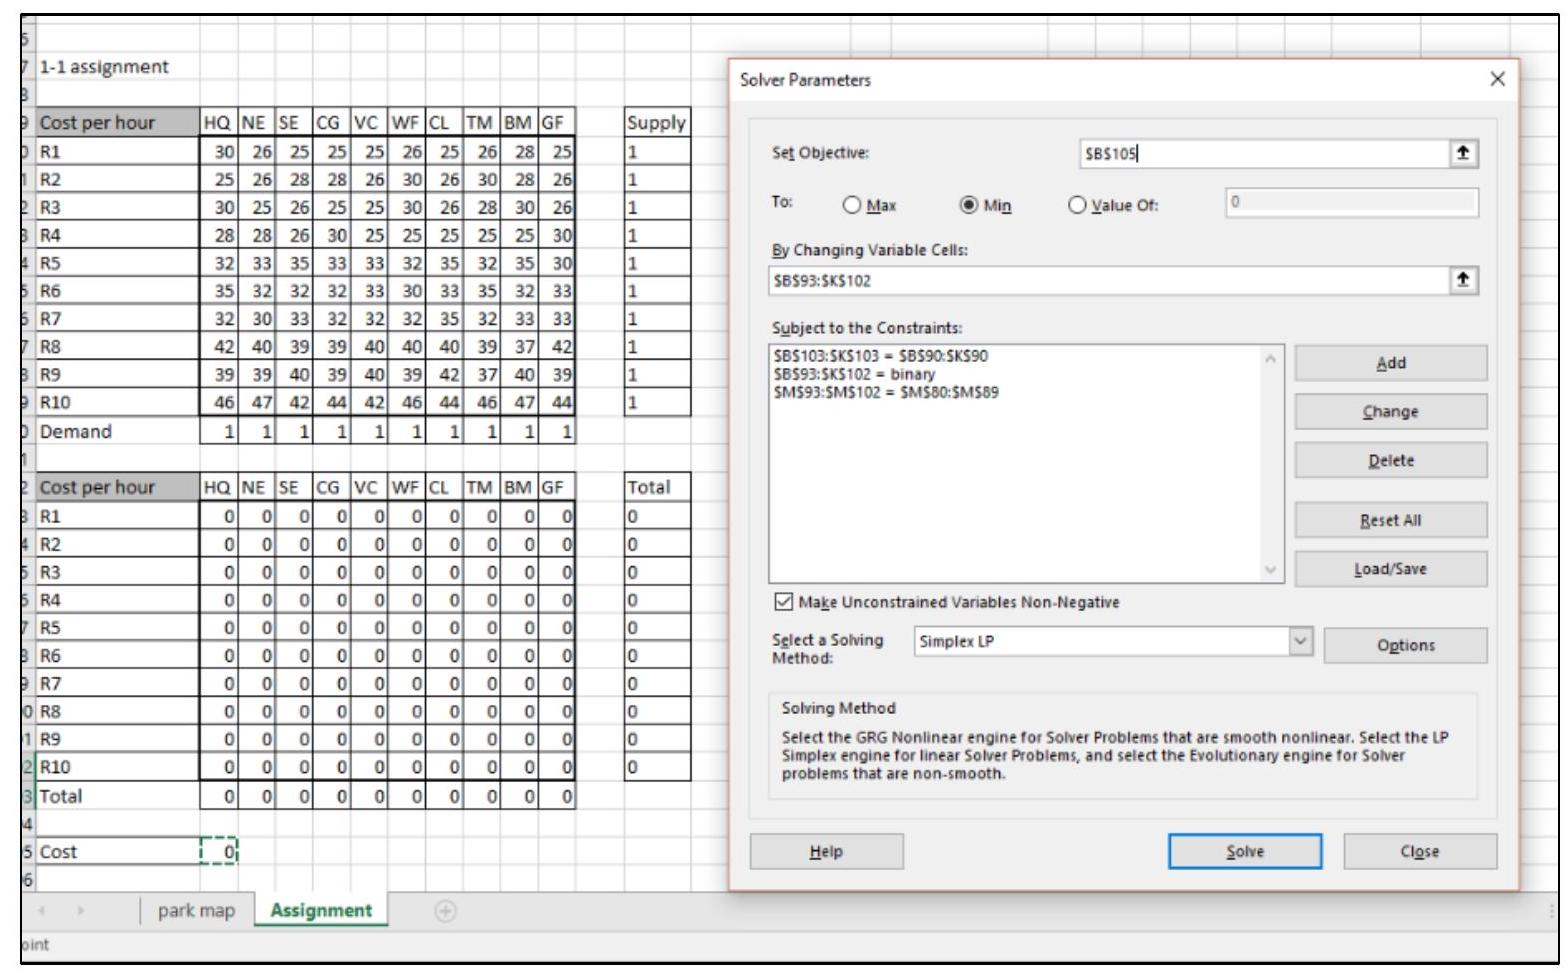
\includegraphics[width=0.5\textwidth]{2024_12_09_1e11ad6a3005a73458cag-06}

\begin{center}
\begin{tabular}{|l|c|c|c|c|c|c|c|c|c|c|}
\hline
Cost per hour & HQ & NE & SE & CG & VC & WF & CL & TM & BM & GF \\
\hline
R1 & 0 & 0 & 1 & 0 & 0 & 0 & 0 & 0 & 0 & 0 \\
\hline
R2 & 1 & 0 & 0 & 0 & 0 & 0 & 0 & 0 & 0 & 0 \\
\hline
R3 & 0 & 0 & 0 & 1 & 0 & 0 & 0 & 0 & 0 & 0 \\
\hline
R4 & 0 & 0 & 0 & 0 & 0 & 0 & 1 & 0 & 0 & 0 \\
\hline
R5 & 0 & 0 & 0 & 0 & 0 & 0 & 0 & 0 & 0 & 1 \\
\hline
R6 & 0 & 0 & 0 & 0 & 0 & 1 & 0 & 0 & 0 & 0 \\
\hline
R7 & 0 & 1 & 0 & 0 & 0 & 0 & 0 & 0 & 0 & 0 \\
\hline
R8 & 0 & 0 & 0 & 0 & 0 & 0 & 0 & 0 & 1 & 0 \\
\hline
R9 & 0 & 0 & 0 & 0 & 0 & 0 & 0 & 1 & 0 & 0 \\
\hline
R10 & 0 & 0 & 0 & 0 & 1 & 0 & 0 & 0 & 0 & 0 \\
\hline
Total & 1 & 1 & 1 & 1 & 1 & 1 & 1 & 1 & 1 & 1 \\
\hline
\end{tabular}
\end{center}

\begin{center}
\begin{tabular}{|l|}
\hline
Total \\
\hline
1 \\
\hline
1 \\
\hline
1 \\
\hline
1 \\
\hline
1 \\
\hline
1 \\
\hline
1 \\
\hline
1 \\
\hline
1 \\
\hline
1 \\
\hline
\end{tabular}
\end{center}

\begin{center}
\begin{tabular}{|l|l|}
\hline
Cost & 306 \\
\hline
\end{tabular}
\end{center}

If we had more rangers than needed, we would again add a placeholder column "not needed" and assign one of the rangers to it. If we had too few rangers, one of the locations would not get staffed, i.e. we'd have an option "not staffed" as an additional row.

\section*{Stating the Solution}
To minimize cost, rangers and volunteers should be assigned as follows (assuming exactly enough volunteers:

\begin{center}
\begin{tabular}{lr}
R1 $\rightarrow$ SE & Assign the 120 NE volunteer hours as follows: 100 hours to WF, 20 hours to CL \\
R2 $\rightarrow$ HQ & Assign the 200 SE volunteer hours as follows: 30 hours to SE, 150 hours to GF \\
R3 $\rightarrow$ CG & Assign the 300 NE volunteer hours as follows: 50 hours to HQ, 30 hours to NE, \\
R4 $\rightarrow$ CL & 50 hours to CG, 100 hours to VC, 20 hours to BM, and 50 hours to GF \\
R5 $\rightarrow$ GF &  \\
R6 $\rightarrow$ WF &  \\
R7 $\rightarrow$ NE &  \\
R8 $\rightarrow$ BM &  \\
R9 $\rightarrow$ TM &  \\
R10 $\rightarrow$ VC &  \\
\end{tabular}
\end{center}

The total cost is $\$ 6,710$ / hour for the volunteers and $\$ 306$ / hour for the rangers.

Note that a similar set-up could be used to instead focus on worker preferences for assignments, their suitability for a task by ranking them, the driving distance to locations, or including urgency of assignments.

\section*{Part 2: Shuttle service - Shortest Path and Maximum Flow}
We will examine two questions:

\begin{enumerate}
  \item What is the shortest route in terms of time from $H Q$ to GF and
  \item Given the limited capacity of the narrow roads in the park, what is the maximum number of shuttle busses we can get from HQ to GF per hour? How much is it going to cost us? And how many visitors can we transport per hour?
\end{enumerate}

We will refer to the table on the next page listing distance, drive time, and capacity for each road segment in the park. Assume that driving time is the same in either direction, and that capacity is as well (i.e. we can run the full capacity in each direction). Instead of minimizing time, one could choose to maximize profit, maximize popularity, or minimize miles driven or incorporate constraints such as parking available at different locations or one-way roads.

\section*{Shortest Path}
\begin{center}
\begin{tabular}{|c|c|c|c|c|}
\hline
From & To & Miles & Minutes & Capacity \\
\hline
\multirow[t]{4}{*}{HQ} & NE & 15 & 20 & 30 \\
\hline
 & WF & 20 & 30 & 20 \\
\hline
 & CG & 5 & 15 & 10 \\
\hline
 & SE & 13 & 22 & 30 \\
\hline
\multirow[t]{2}{*}{NE} & HQ & 15 & 20 & 30 \\
\hline
 & WF & 12 & 30 & 15 \\
\hline
\multirow[t]{4}{*}{CG} & HQ & 5 & 15 & 10 \\
\hline
 & SE & 7 & 14 & 10 \\
\hline
 & VC & 5 & 20 & 5 \\
\hline
 & WF & 9 & 15 & 8 \\
\hline
\multirow[t]{3}{*}{SE} & HQ & 13 & 22 & 30 \\
\hline
 & CG & 7 & 14 & 10 \\
\hline
 & VC & 22 & 25 & 30 \\
\hline
\multirow[t]{6}{*}{vC} & SE & 22 & 25 & 30 \\
\hline
 & CG & 5 & 20 & 5 \\
\hline
 & WF & 15 & 30 & 9 \\
\hline
 & FCP & 8 & 15 & 5 \\
\hline
 & GF & 32 & 45 & 20 \\
\hline
 & BM & 16 & 20 & 30 \\
\hline
\multirow[t]{6}{*}{WF} & NE & 12 & 30 & 15 \\
\hline
 & HQ & 20 & 30 & 20 \\
\hline
 & CG & 9 & 15 & 8 \\
\hline
 & VC & 15 & 30 & 9 \\
\hline
 & FCP & 5 & 15 & 3 \\
\hline
 & CL & 15 & 20 & 12 \\
\hline
\multirow[t]{4}{*}{FCP} & WF & 5 & 15 & 3 \\
\hline
 & VC & 8 & 15 & 5 \\
\hline
 & TM & 10 & 15 & 6 \\
\hline
 & CL & 11 & 15 & 8 \\
\hline
\multirow[t]{4}{*}{CL} & WF & 15 & 20 & 12 \\
\hline
 & FCP & 11 & 15 & 8 \\
\hline
 & TM & 4 & 20 & 2 \\
\hline
 & GF & 16 & 28 & 8 \\
\hline
\multirow[t]{3}{*}{TM} & FCP & 10 & 15 & 6 \\
\hline
 & CL & 4 & 20 & 2 \\
\hline
 & GF & 3 & 15 & 2 \\
\hline
\multirow[t]{2}{*}{BM} & VC & 16 & 20 & 30 \\
\hline
 & GF & 20 & 30 & 15 \\
\hline
\multirow[t]{4}{*}{GF} & CL & 16 & 28 & 8 \\
\hline
 & TM & 3 & 15 & 2 \\
\hline
 & vC & 32 & 45 & 20 \\
\hline
 & BM & 20 & 30 & 15 \\
\hline
\end{tabular}
\end{center}

To find the shortest path from HQ to GF, we can start by deleting all the roads that are not needed. For example, if we start at HQ, we will not go back from NE to HQ. Similarly, once we reach GF, we are done and do not need to leave again. This step is not strictly necessary to solve our small problem, but it is good form.

We will adopt terminology you may be familiar with from Discrete Structure. What we have here is a network problem. A network consists of nodes or vertices, the locations, and arcs, the roads. A (directed) path from $A$ to $B$ is a sequence of connecting arcs where the direction is from $A$ to $B$. The out-degree, deg $^{+}$of a node is the number of arcs originating at that node (leaving). The in-degree, deg; of a node is the number of arcs terminating at that node (entering). The net flow is deg $^{+}$- deg. For our first question, we are looking for a shortest path from HQ to GF.

Because HQ is our start point, we want it to have a net flow of 1 . Our end point, GF, needs to have a net flow of -1, while all other nodes are either intermediate nodes or not used at all, so they all have zero net flow. You should convince yourself that this set-up guarantees a connected path from HQ to GF.

This problem can again be framed as a Linear Programming problem. We have a linear objective function to minimize, namely the sum of the times needed for all chosen paths. The decision variables, one for each path, have just two values. We set them $=1$ if the path is chosen, and $=0$ otherwise.

To compute net flow, we use the Sumlf function. The Sumlf function checks range\_1 for any value that meets the criteria, and if it finds them adds up the corresponding entries in the sum\_range.

Syntax: =Sumlf(range\_1, criteria, sum\_range)

For details on how to set up the work sheet, refer to the screenshot below. There are two important things: First of all, the decision variables need to be constraint to be binary. That way, we avoid partial roads, which make no sense. Second, it is important to hold the ranges in the "Sumlf" statement fixed (use F4 key or \$\$ signs)\\
\begin{center}
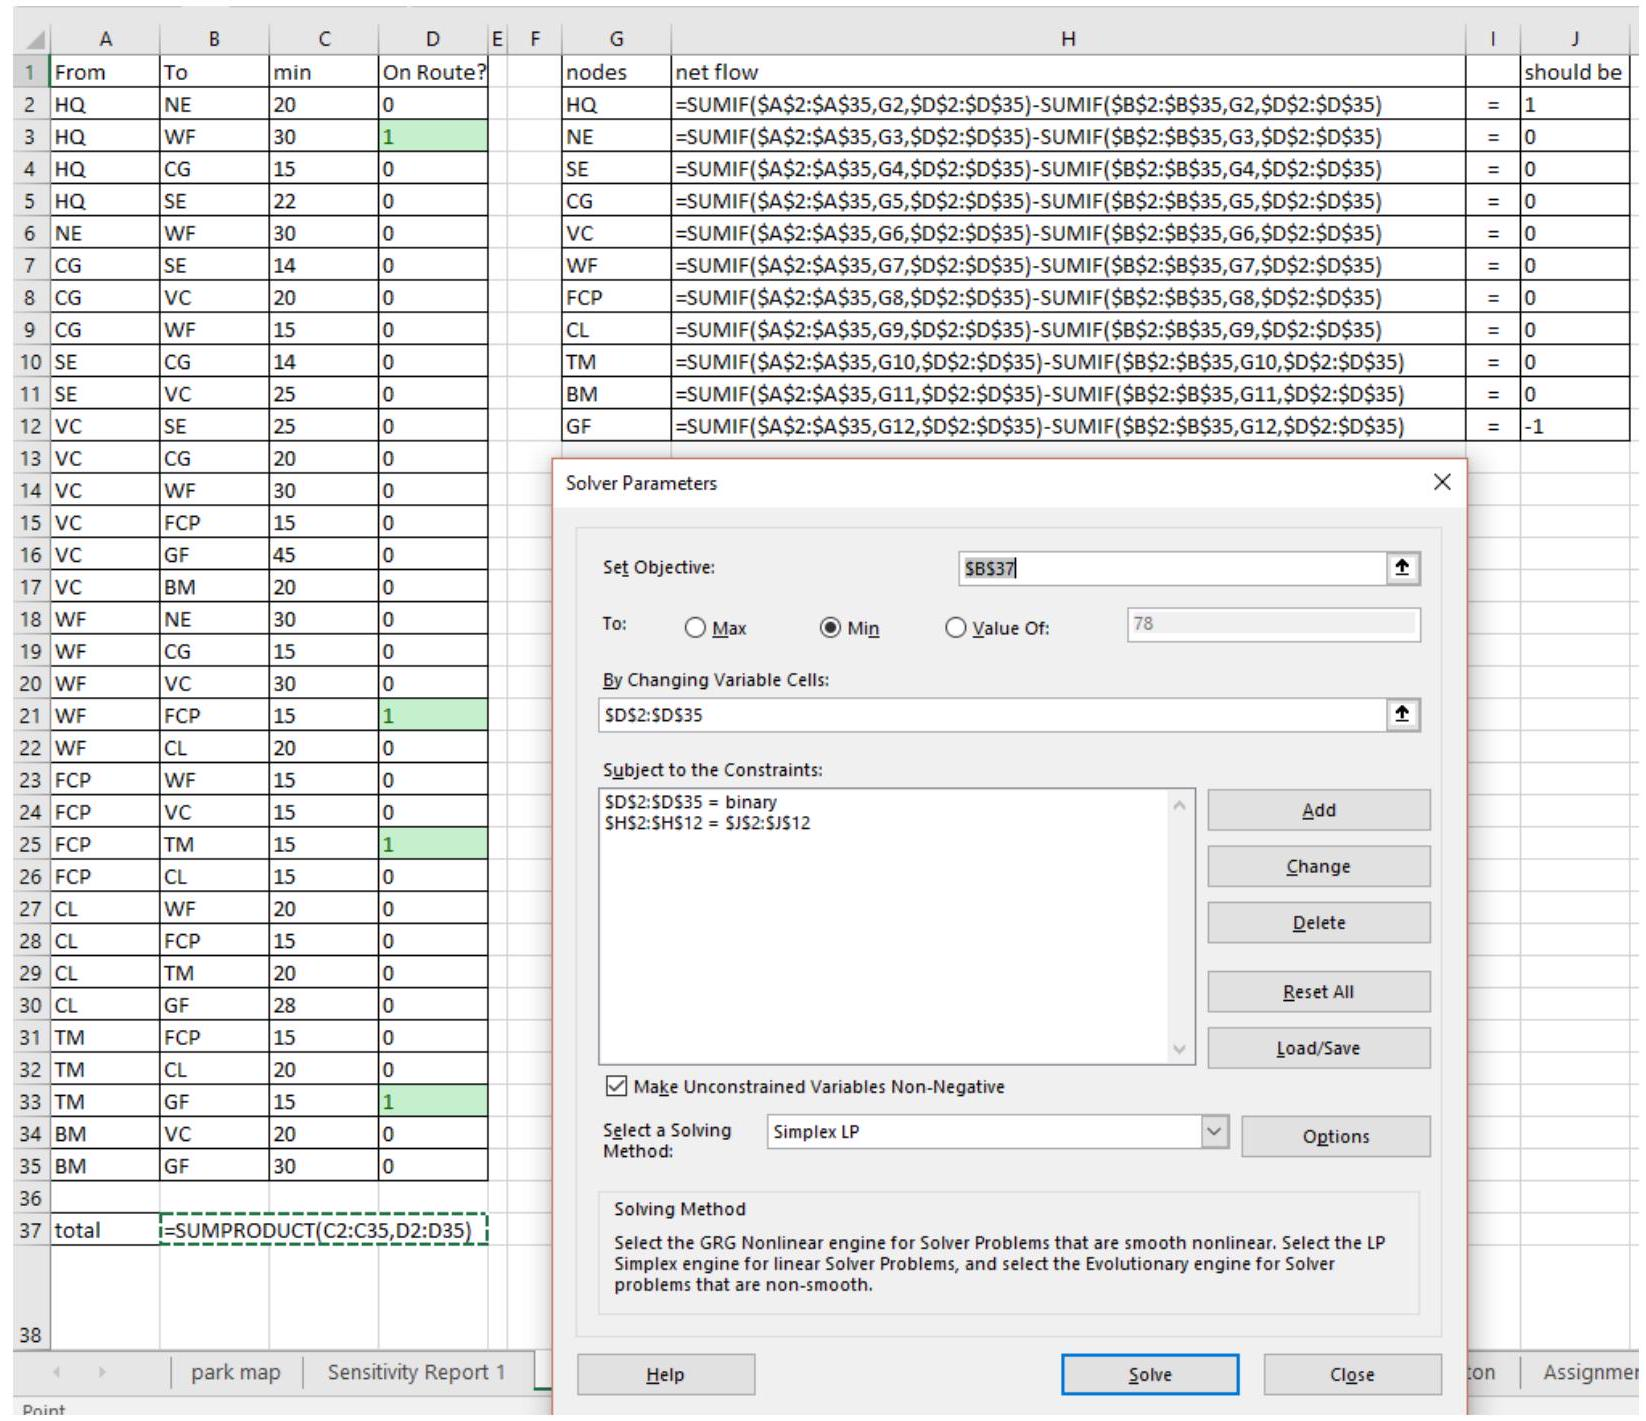
\includegraphics[width=0.7\textwidth]{2024_12_09_1e11ad6a3005a73458cag-09}
\end{center}

\section*{Stating the Solution}
The solution turns out $\mathrm{HQ} \rightarrow \mathrm{WF} \rightarrow \mathrm{FCP} \rightarrow \mathrm{TM} \rightarrow \mathrm{GF}$ for a total of 75 minutes driving time. This is the shortest path (in terms of time) available. As far as the capacity is concerned, we need to use the minimum capacity for any of the four legs, which is 2 for TM to GF.

\section*{Maximum Flow}
Two shuttles are not much, we will probably need more. How many shuttle busses total could we get from HQ to GF? And how can we do that with minimum total time? This question really asks us to solve\\
a problem with two objective functions: Maximize flow while minimizing total time. To answer that question, we look at our park map, this time annotated with the capacities.\\
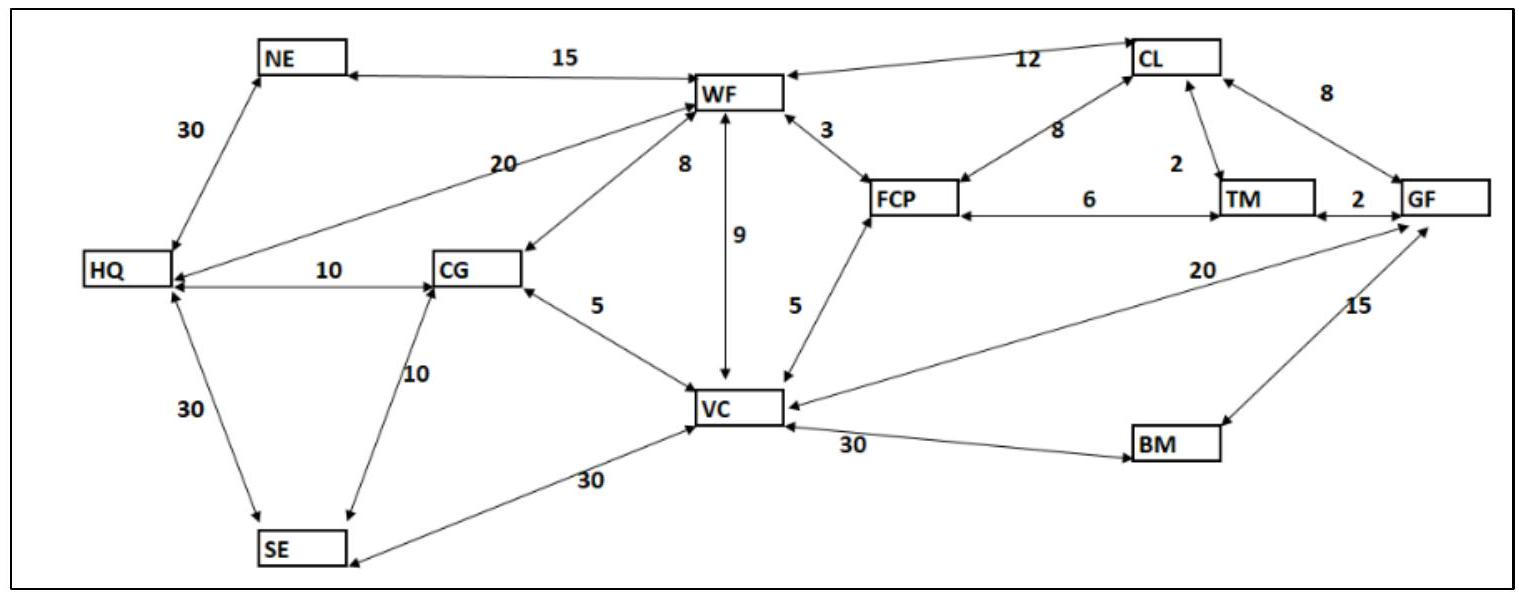
\includegraphics[width=0.9\textwidth]{2024_12_09_1e11ad6a3005a73458cag-10(2)}

We already run 2 shuttles on $\mathrm{HQ} \rightarrow \mathrm{WF} \rightarrow \mathrm{FCP} \rightarrow \mathrm{TM} \rightarrow \mathrm{GF}$, so we change the numbers to reflect capacities still available. In effect, the road from TM to GF is no longer available. We eliminate that option from our list. (line 33).\\
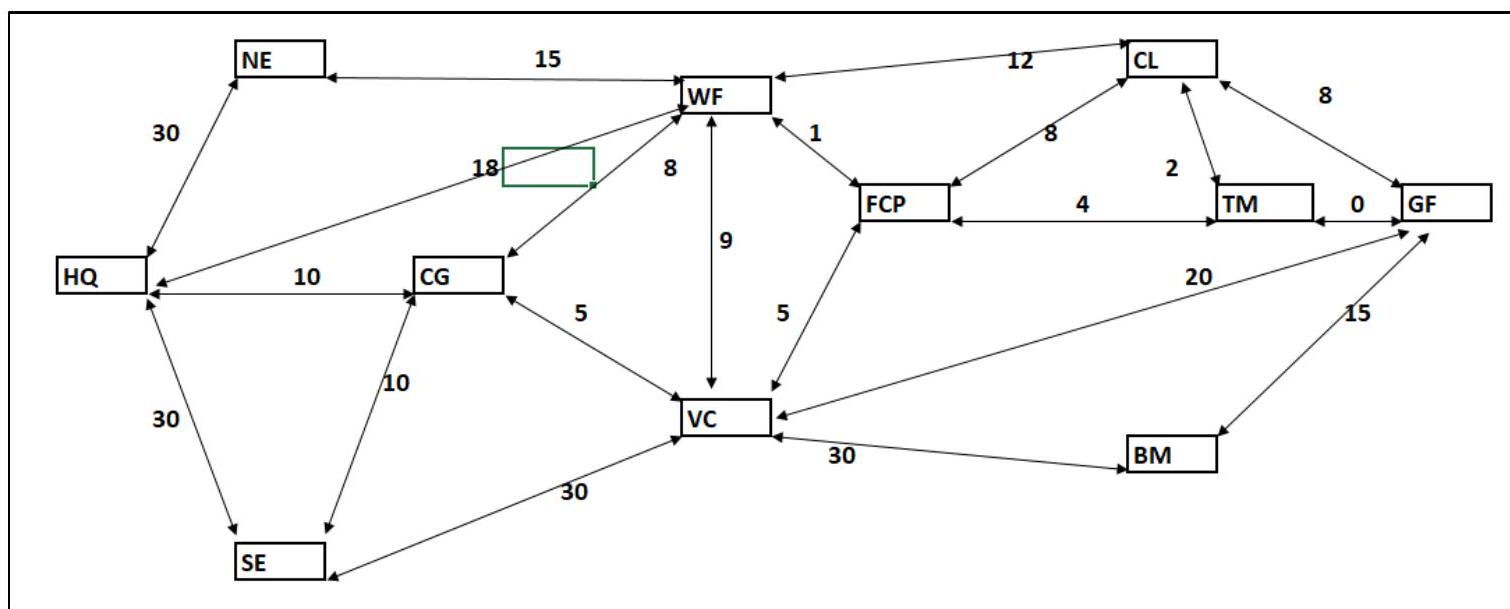
\includegraphics[width=0.5\textwidth]{2024_12_09_1e11ad6a3005a73458cag-10(1)}

Running the shortest path problem again (with one road less) gives us the path $H Q \rightarrow W F \rightarrow C L \rightarrow F \rightarrow G F$, with 78 minutes. This route will accommodate 8 additional shuttles. We again adjust our map and table to reflect that yet another route is maxed out.\\
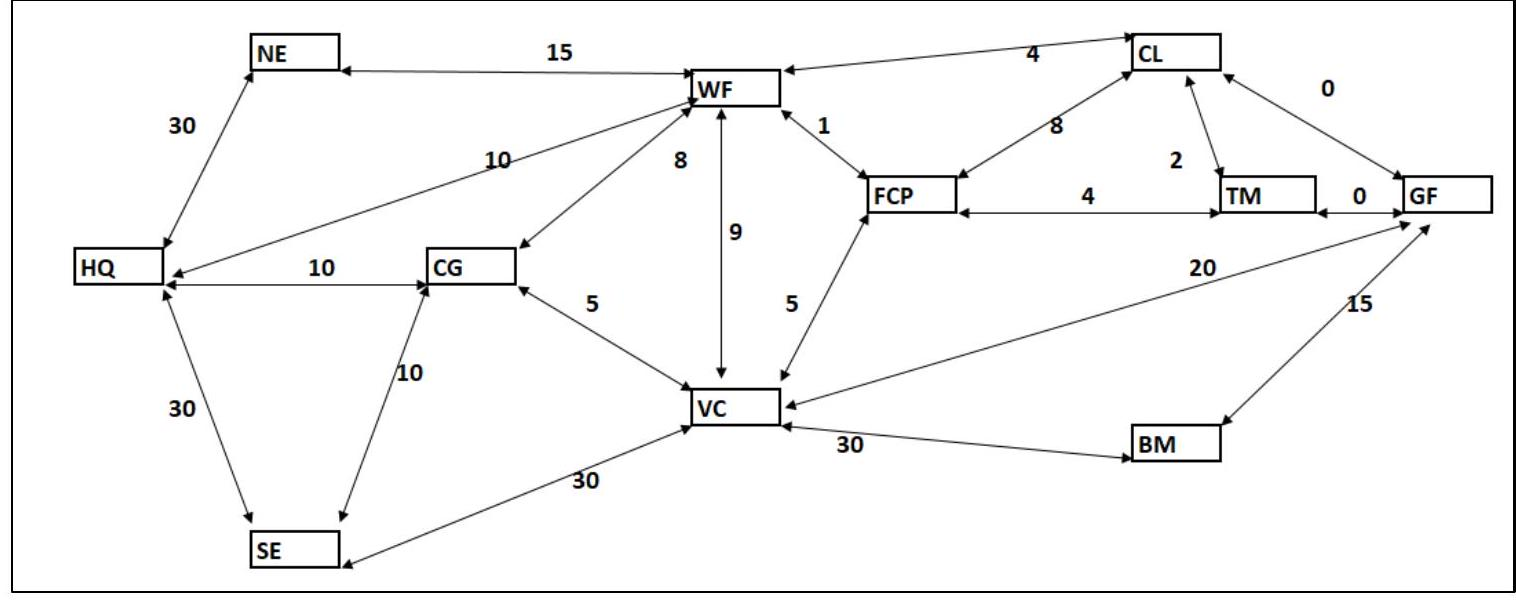
\includegraphics[width=0.9\textwidth]{2024_12_09_1e11ad6a3005a73458cag-10}

We continue alternating the shortest path problem with adjusting route list and map, and arrive at the solution:

\begin{center}
\begin{tabular}{|l|l|l|}
\hline
route & time & capacity \\
\hline
$\mathrm{HQ} \rightarrow \mathrm{WF} \rightarrow \mathrm{FCP} \rightarrow \mathrm{TM} \rightarrow \mathrm{GF}$ & 75 & 2 \\
\hline
$\mathrm{HQ} \rightarrow \mathrm{WF} \rightarrow \mathrm{CL} \rightarrow \mathrm{GF}$ & 78 & 8 \\
\hline
$\mathrm{HQ} \rightarrow \mathrm{CG} \rightarrow \mathrm{VC} \rightarrow \mathrm{GF}$ & 80 & 5 \\
\hline
$\mathrm{HQ} \rightarrow \mathrm{SE} \rightarrow \mathrm{VC} \rightarrow \mathrm{GF}$ & 92 & 15 \\
\hline
$\mathrm{HQ} \rightarrow \mathrm{SE} \rightarrow \mathrm{VC} \rightarrow \mathrm{BM} \rightarrow \mathrm{GF}$ & 97 & 15 \\
\hline
 & Average time $\approx 89 \mathrm{~min}$ & Total shuttles: 45 \\
\hline
\end{tabular}
\end{center}

This is an example of a greedy algorithm. In each iteration, we pick what is best without considering the impact on future iterations. A greedy algorithm may, depending on the problem, have the effect that each iteration gives the optimal result given the previous iterations, but not necessarily the best result overall.

Following is a different, two-step approach. First, we solve the maximum flow problem without cost concerns. We use the max capacity as one of our constraints and allow the decision variables to be integers. The net flow is restricted only for the transitional nodes.\\
\begin{center}
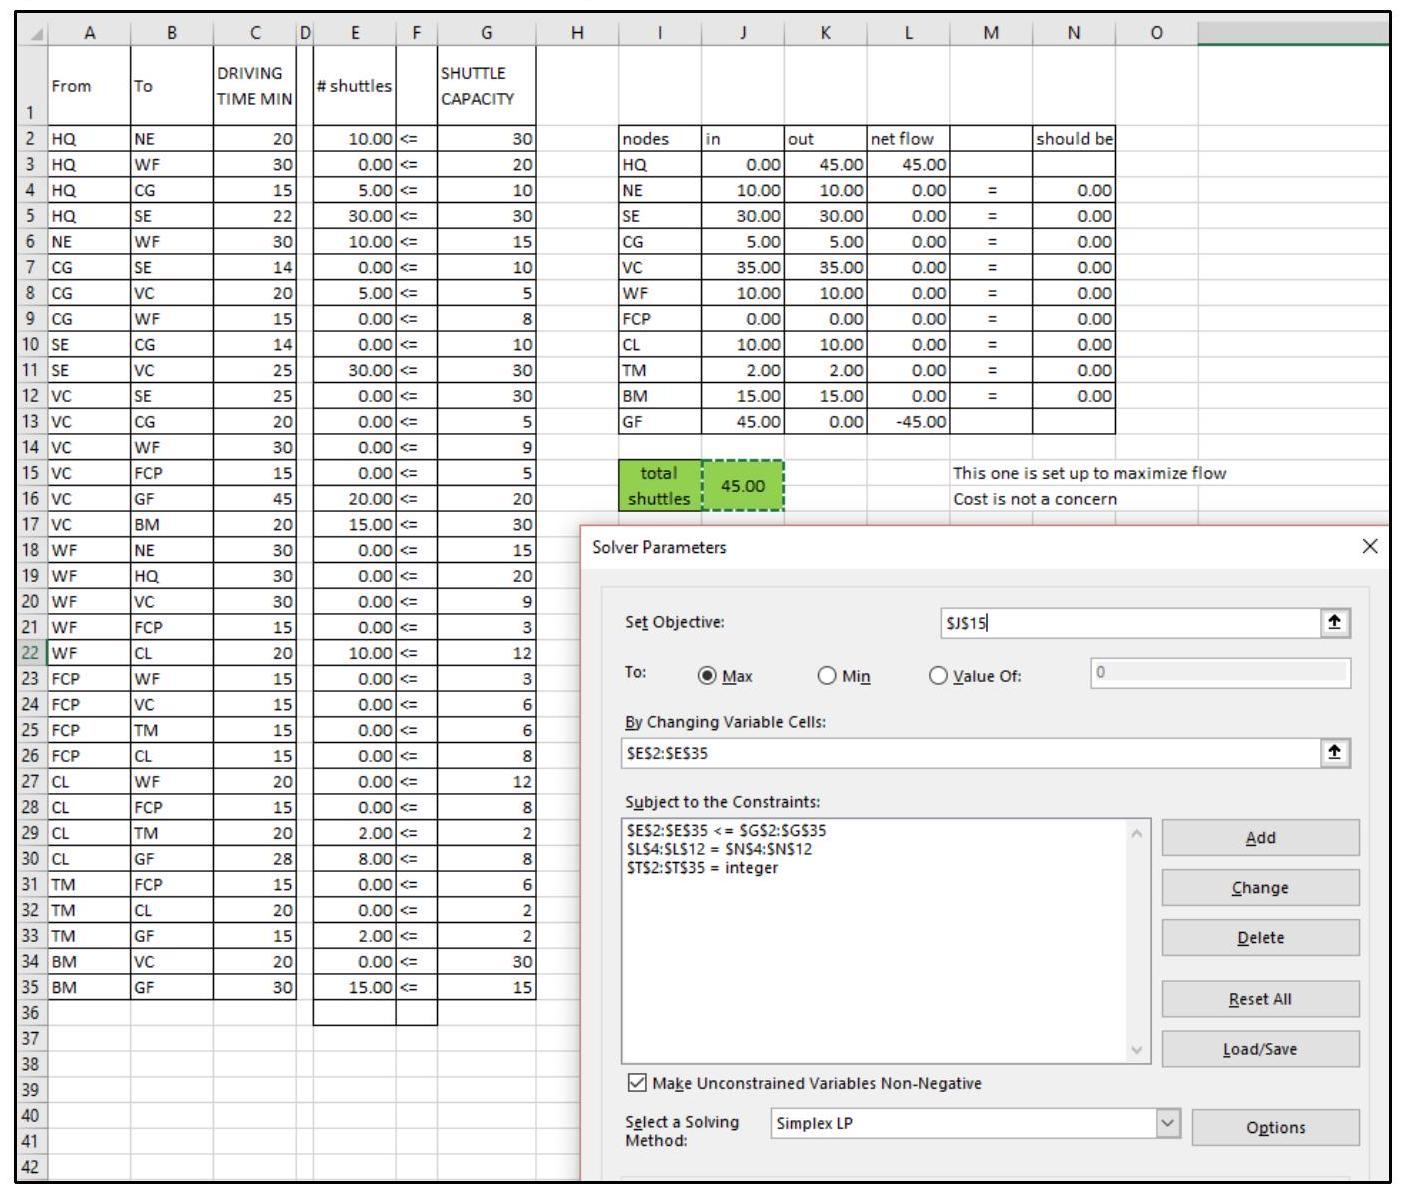
\includegraphics[width=0.7\textwidth]{2024_12_09_1e11ad6a3005a73458cag-11}
\end{center}

We find that the maximum possible flow is 45 , just as before. Next, we can address cost (time).

\section*{Maximum Flow - Minimum Cost}
To solve the maximum flow problem with cost constraints we use the result from the last section and modify the minimum cost problem. We set the netflow for our start point, HQ , to the maximum capacity and the netflow of our end point, GF, to the negative maximum capacity. Of course, we also change the objective function.\\
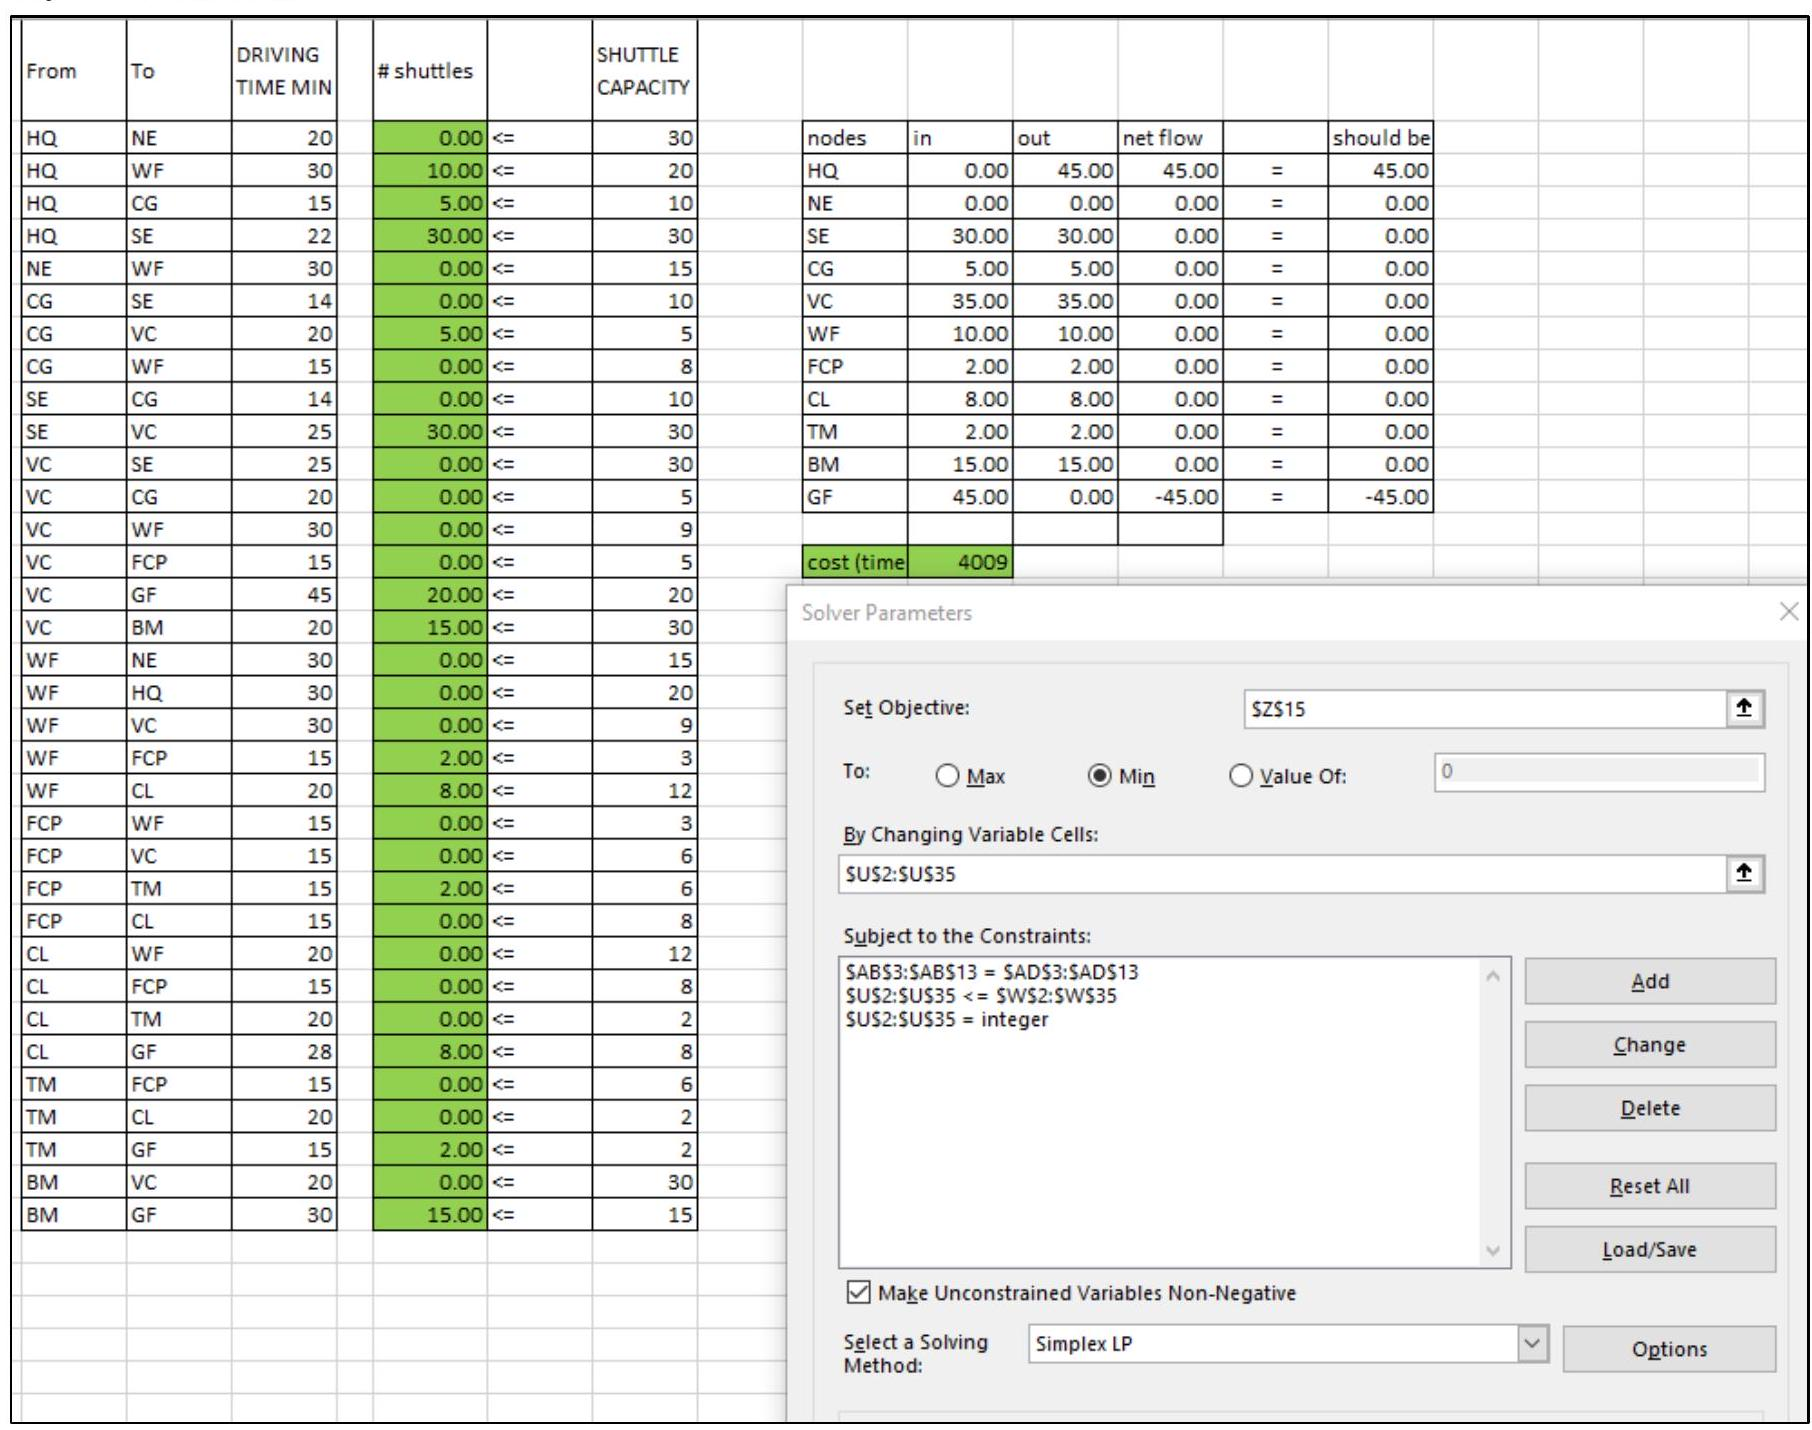
\includegraphics[width=0.9\textwidth]{2024_12_09_1e11ad6a3005a73458cag-12}

The average time needed is the same as before, $\approx 90$ minutes per shuttle. Note that you could use this last set-up to find the lowest average time for any number of shuttles, as long as the total stays at or below capacity.

While the total number of shuttles and the time needed is the same for both approaches, the routes taken are different. This is common for maximum flow problems. In fact, if you choose to solve a maximum flow problem by hand, it does not matter which route you start with.

\section*{Stating the Solution}
If we use 50 passenger busses, we can transport 2250 passengers per hour using the maximum possible 45 shuttles per hour leaving HQ. Given that the roundtrip takes and average 90 minutes, and allowing 90 minutes at GF for sightseeing, this probably means we should start leaving HQ at 8 am and have the last shuttle leave no later than 4 pm . This means we need 135 busses and can transport 18,000 passengers per day. This may not be enough (given that, for example, Yellowstone sees 900,000+ visitors in July). We may have to consider bigger busses, wider roads, or restricting visitor numbers.

\section*{Part 3: Plowing - Minimum Spanning Tree}
This problem is an example of a minimum spanning tree problem. A minimum spanning tree is a subset of a connected, weighted, undirected graph that connects all the nodes together in such a way that the total arc weight (cost) is minimized. There can be no cycles or loops, otherwise the tree would not be minimal.

Our plowing contractor charges by the mile, so we are trying to minimize distance, not driving time. Each road needs two passes, one in each direction. Here again a greedy algorithm works. Start with a graph showing all the locations (nodes), roads (arcs), and distances (weights). Build the tree by including the shortest roads first, but only if they do not create any loops. Add the next shortest roads, again watching out for loops. Continue until you have a connected tree.\\
We will add roads $\mathrm{TM} \rightarrow \mathrm{GF}(3), \mathrm{CL} \rightarrow \mathrm{TM}(4), \mathrm{WF} \rightarrow \mathrm{CL}(5), \mathrm{HQ} \rightarrow \mathrm{CG}(5), \mathrm{CG} \rightarrow \mathrm{VC}$ (5) successively.\\
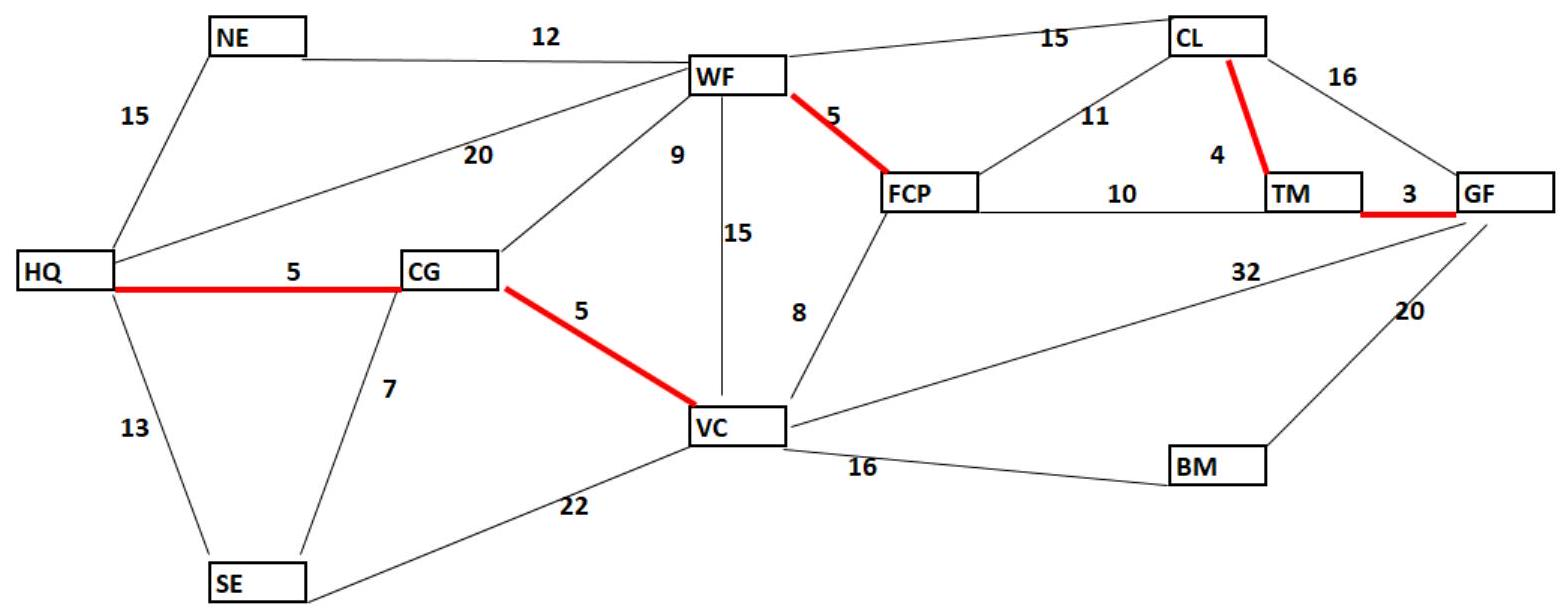
\includegraphics[width=0.5\textwidth]{2024_12_09_1e11ad6a3005a73458cag-13}

Next are $\mathrm{SE} \rightarrow \mathrm{CG}$ (7) and $\mathrm{VC} \rightarrow \mathrm{FCP}$ (8), but not $\mathrm{CG} \rightarrow \mathrm{WF}$ (9) which would create a loop. We can add $\mathrm{TM} \rightarrow \mathrm{FCP}$ (10), but not $\mathrm{FCP} \rightarrow \mathrm{CL}$ (11).\\
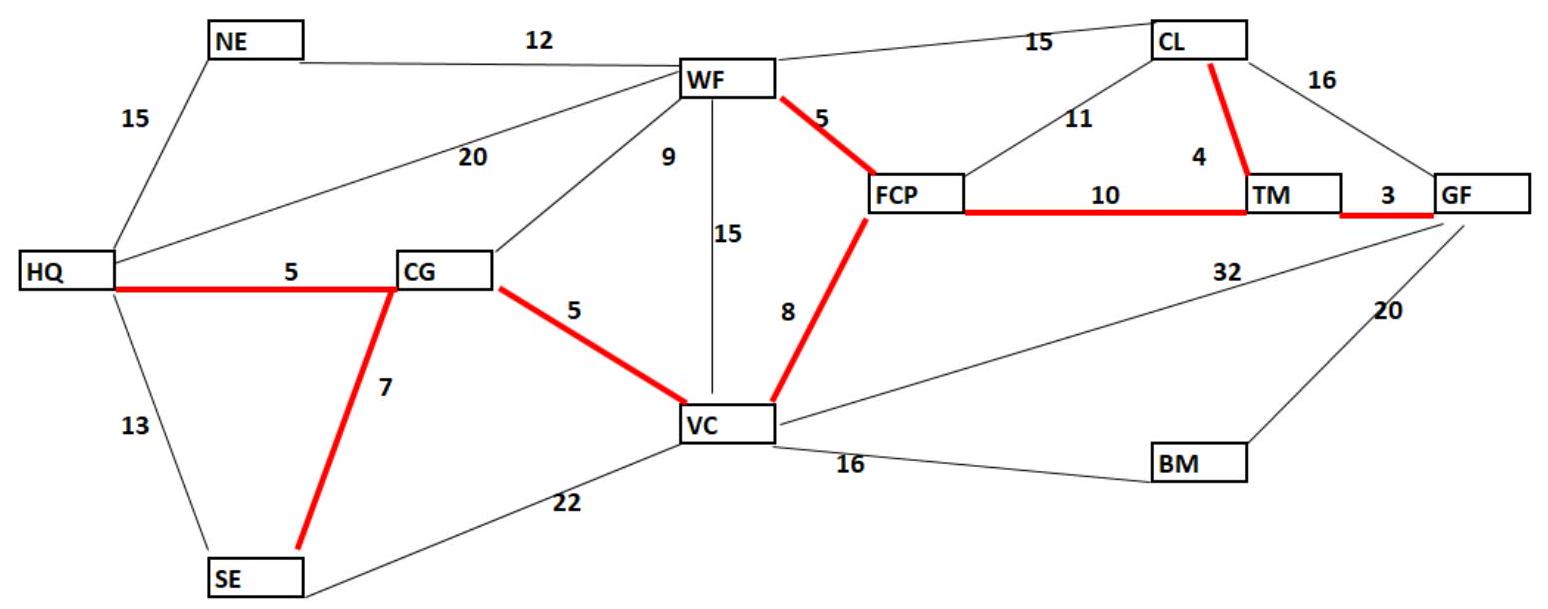
\includegraphics[width=0.5\textwidth]{2024_12_09_1e11ad6a3005a73458cag-14}

Finally, we add $W F \rightarrow N E$ (12) and $V C \rightarrow B M$ (16), for a total of 75 miles of road or 150 miles of plowing.\\
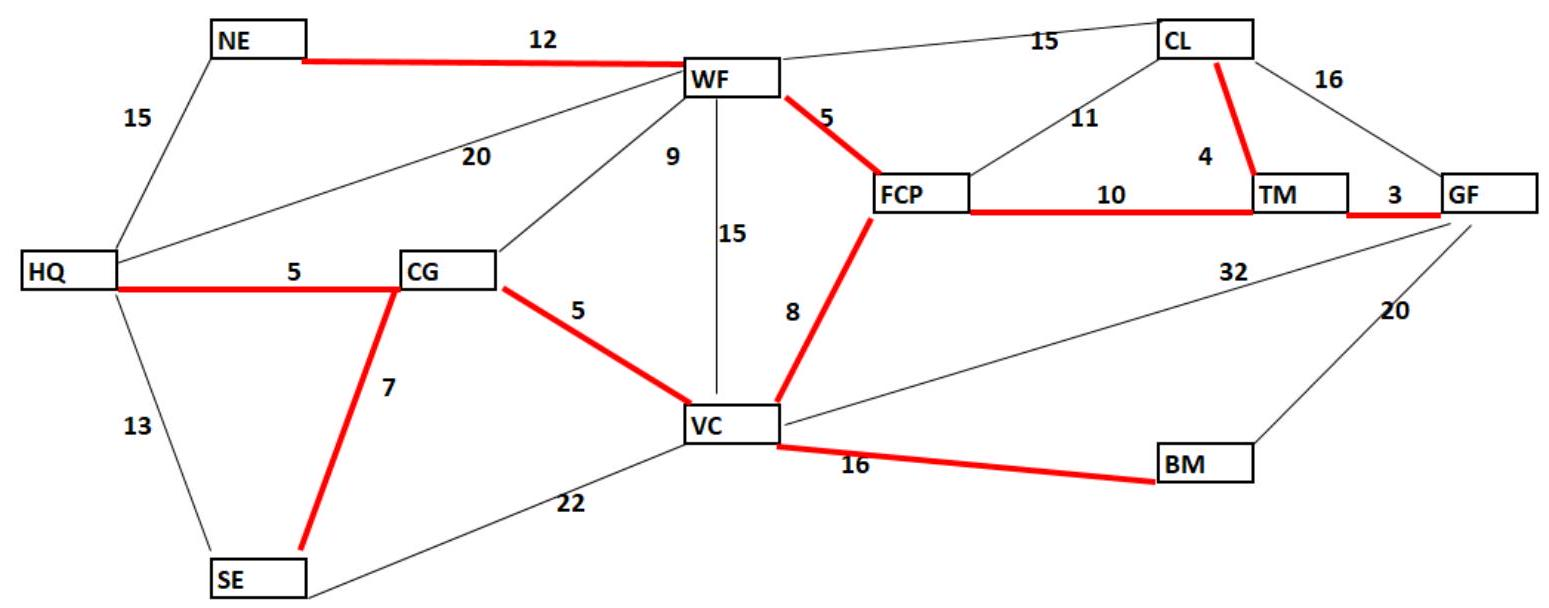
\includegraphics[width=0.5\textwidth]{2024_12_09_1e11ad6a3005a73458cag-14(1)}

This also tells us which roads can be closed in winter. Because we found a spanning tree, the contractor can start and end at any location or entrance.

\section*{Stating the Solution}
To minimize cost, the following roads should be plowed:\\
$\mathrm{TM} \rightarrow \mathrm{GF}, \mathrm{CL} \rightarrow \mathrm{TM}, \mathrm{WF} \rightarrow \mathrm{CL}, \mathrm{HQ} \rightarrow \mathrm{CG}, \mathrm{CG} \rightarrow \mathrm{VC}, \mathrm{WF} \rightarrow \mathrm{NE}, \mathrm{SE} \rightarrow \mathrm{CG}, \mathrm{VC} \rightarrow \mathrm{FCP}, \mathrm{TM} \rightarrow \mathrm{FCP}$, and VC $\rightarrow \mathrm{BM}$, for a total of 150 miles of plowing. Contractors located at any of the three park entrances can be used with no difference in mileage, so the cheapest option should be used

\section*{Part 4: Deliveries - Traveling Salesman Problem}
Assume you need to deliver supplies to each of the 11 locations in the park, starting and ending at HQ . You want to visit each location exactly once. In graph theory, a path that visits each vertex in a graph exactly once and ends and starts at the same vertex is called a Hamiltonian circuit. The problem of finding the minimum cost such path is called the Traveling Salesman Problem (TSP), probably the most famous problem in OR. This is a notoriously difficult problem to solve efficiently.

There are 11 locations to visit in a circuit. One could attempt to list all possible paths of length 11, pick out the potential solutions (those through all 11 locations), compute the length and pick the best. The problem with this brute force approach is that there are so many possibilities. In the worst-case scenario, i.e. a complete graph with 11 vertices (complete means that each vertex is connected to every other vertex), there are $\frac{(\mathrm{n}-1)!}{2}=\frac{10!}{2}=1,814,400$ possible paths to check. While we do have only 21 edges instead of the 55 of a complete graph, it is still not feasible to find and check all potential paths.

We will use an approach called a heuristic, which is short for heuristic technique. A heuristic is an approach that uses a practical, often intuitive approach to problem solving. It is not guaranteed to yield the optimal result, but instead one that is "good enough" (hopefully),

\section*{Nearest neighbor approach}
The nearest neighbor approach is fast, simple, and often yields a good short path. However, there are instances where it doesn't work at all or even yields the worst path. The idea is to start at an arbitrary vertex, chose the edge to the nearest unconnected vertex, and continue until the circuit is complete. This approach works well if the graph is complete or nearly so. In our case, starting at HQ , we end up "stuck", there is no path from BM back to NE:\\
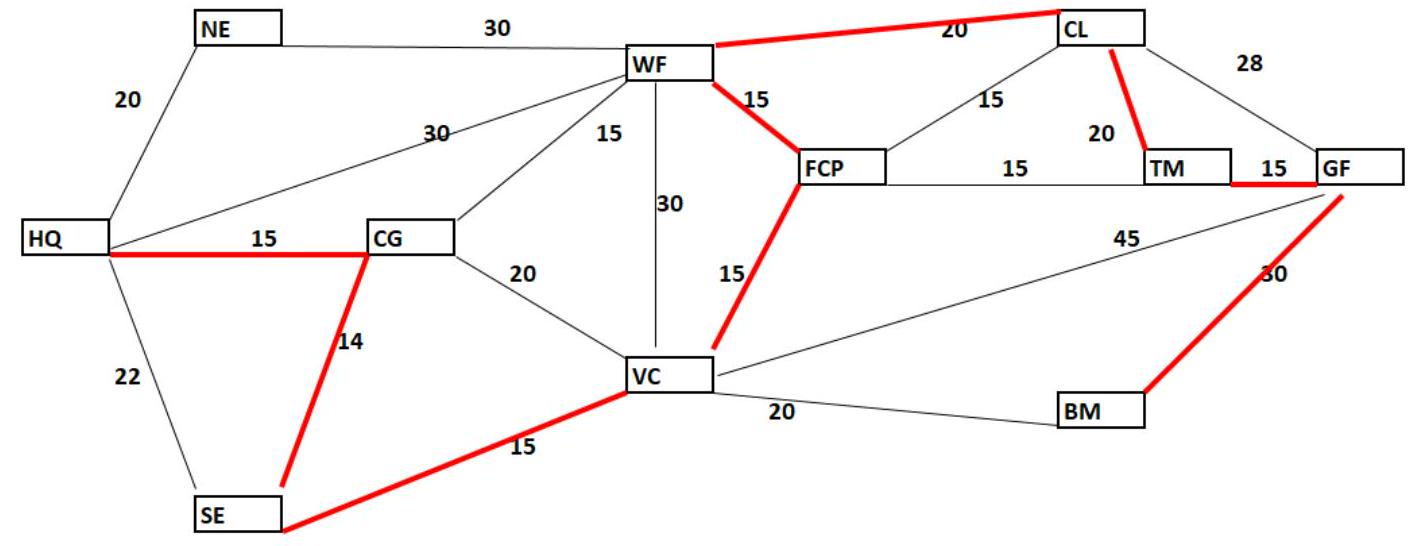
\includegraphics[width=0.5\textwidth]{2024_12_09_1e11ad6a3005a73458cag-15}

You may have noticed that we had choices at FCP, however, each of them will lead to the same problem. There just aren't enough edges.

One way around this is to use a modified nearest neighbor approach. We recognize that there are two nodes, NE and BM, where we do not have a choice how to reach them. We can therefor treat those segments (shown below) as a unit and try the nearest neighbor approach again.\\
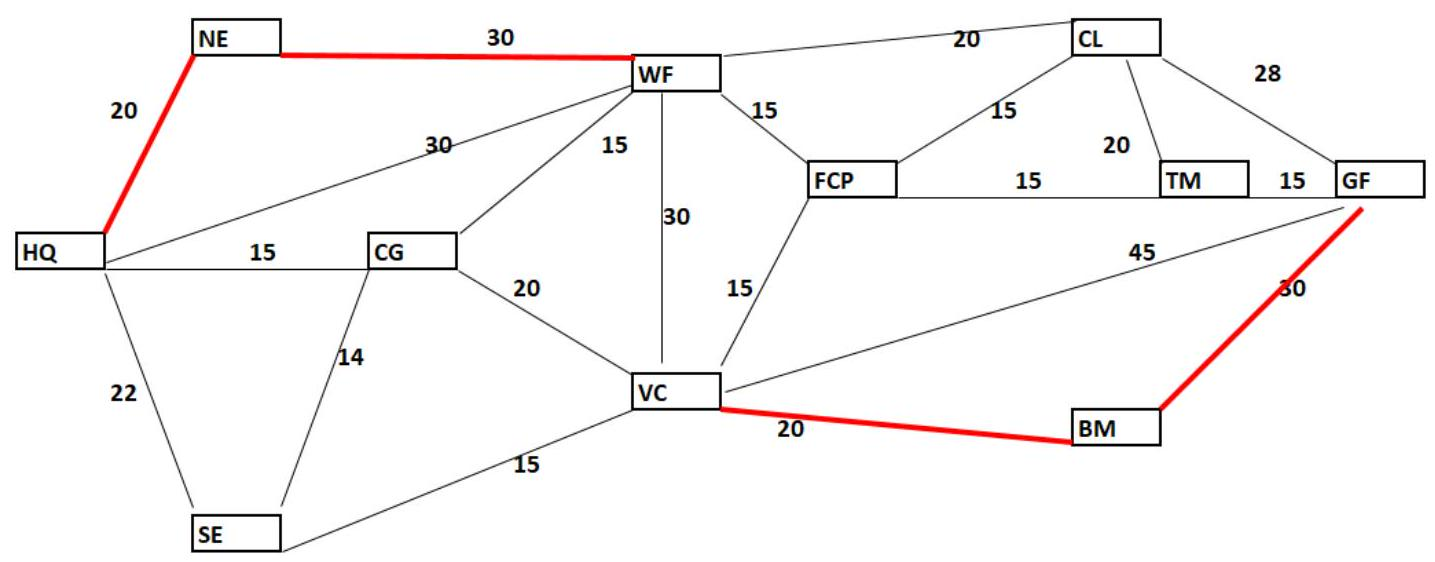
\includegraphics[width=0.5\textwidth]{2024_12_09_1e11ad6a3005a73458cag-16}

Starting at HQ , this time we get a solution. The total length of this circuit is 209.\\
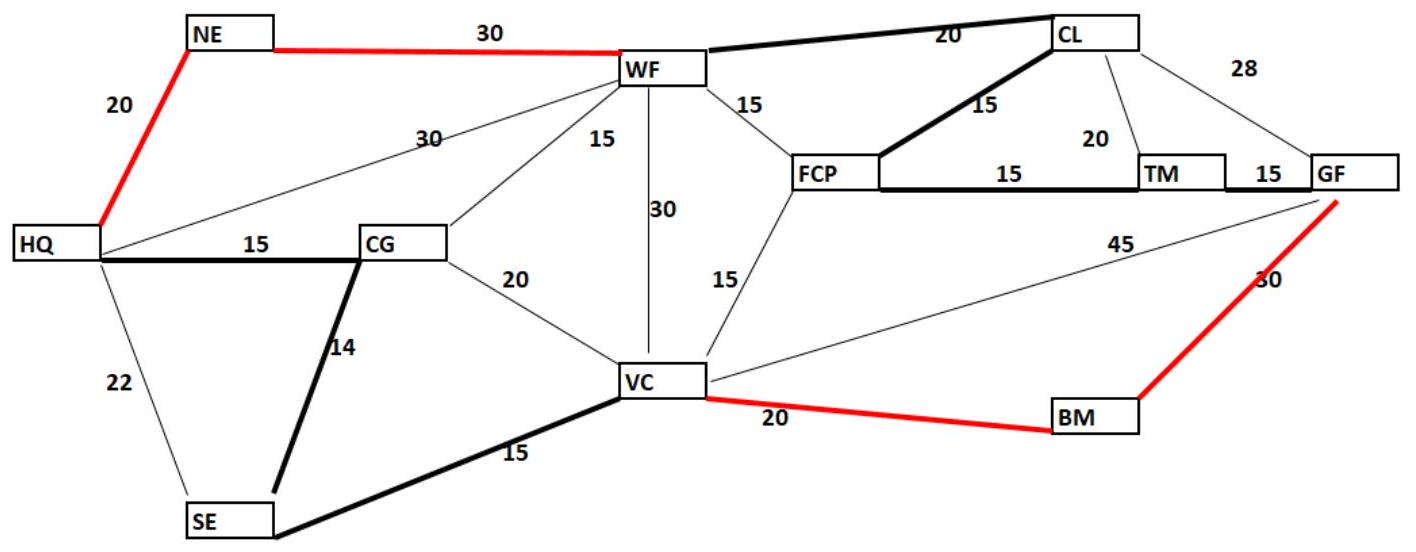
\includegraphics[width=0.5\textwidth]{2024_12_09_1e11ad6a3005a73458cag-16(2)}

\section*{Sub-tour Reversal}
Next, we examine a technique called sub-tour reversal. We start with any possible directed circuit:\\
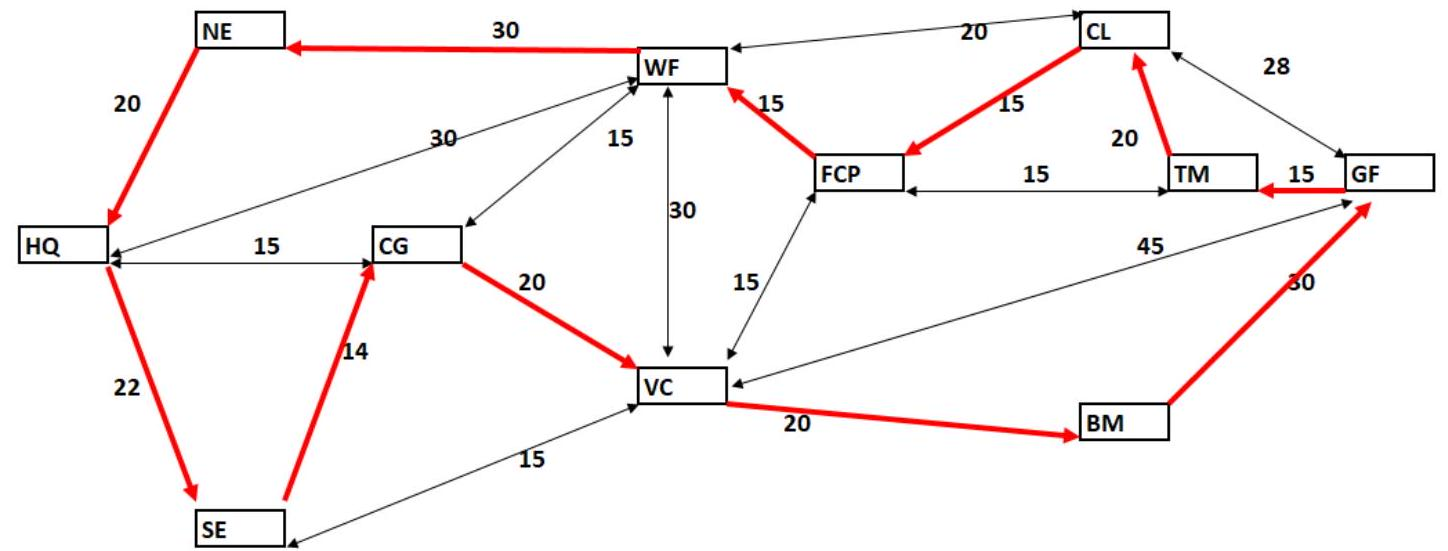
\includegraphics[width=0.5\textwidth]{2024_12_09_1e11ad6a3005a73458cag-16(1)}

This circuit is not - and doesn't have to be - perfect, it just serves as a starting point. The idea is to look at sub-tours, starting with one-segment ones, then two-segments, etc. We will look at each of those sub-tours and check if the total cost can be improved if we reverse direction. If we reverse direction, it will also affect the two path segments directly adjacent. We again start at HQ.

\begin{center}
\begin{tabular}{|c|c|}
\hline
HQ $\rightarrow$ SE & If we reverse $\mathrm{HQ} \rightarrow \mathrm{SE}$, the edges $\mathrm{NE} \rightarrow \mathrm{HQ}$ and $\mathrm{SE} \rightarrow \mathrm{CG}$ no longer work (left graph). We can add $\mathrm{HQ} \rightarrow \mathrm{CG}$, but there is no edge from NE to SE . Without it, the circuit is broken. \\
\hline
SE $\rightarrow$ CG & Reversing $\mathrm{SE} \rightarrow$ CG to CG $\rightarrow$ SE means the adjacent edges, $\mathrm{HQ} \rightarrow \mathrm{SE}$ and $\mathrm{SE} \rightarrow \mathrm{VC}$ no longer work. We replace them with $\mathrm{HQ} \rightarrow \mathrm{CG}$ and $\mathrm{SE} \rightarrow \mathrm{VC}$, respectively. This results in a reduction of cost by 12 . \\
\hline
CG $\rightarrow$ VC & Not possible, can't connect CG to BM \\
\hline
$\mathrm{VC} \rightarrow \mathrm{BM}$ & Not possible, can't connect CG to BM \\
\hline
BM $\rightarrow$ GF & Not possible, can't connect TM to BM \\
\hline
GF $\rightarrow$ TM & Not possible, can't connect TM to BM \\
\hline
$\mathrm{TM} \rightarrow \mathrm{CL}$ & This reversal is possible; however, it results in an increase in cost by 13. \\
\hline
$\mathrm{CL} \rightarrow \mathrm{FCP}$ & This reversal is possible, but it results in no change in total cost. \\
\hline
FCP $\rightarrow$ WF & Not possible, can't connect FCP to NE \\
\hline
WF $\rightarrow$ NE & Not possible, can't connect FCP to NE \\
\hline
$\mathrm{NE} \rightarrow \mathrm{HQ}$ & Not possible, can't connect NE to SE \\
\hline
\end{tabular}
\end{center}

Of all three possible 1-segment subtour reversals, reversing $S E \rightarrow C G$ to $C G \rightarrow$ SE gives the best result, so we will implement that. Next, we check all two-segment sub-tours, then all three-segment sub-tours and so on (it turns out none of those are reversible). Our final circuit looks like this:\\
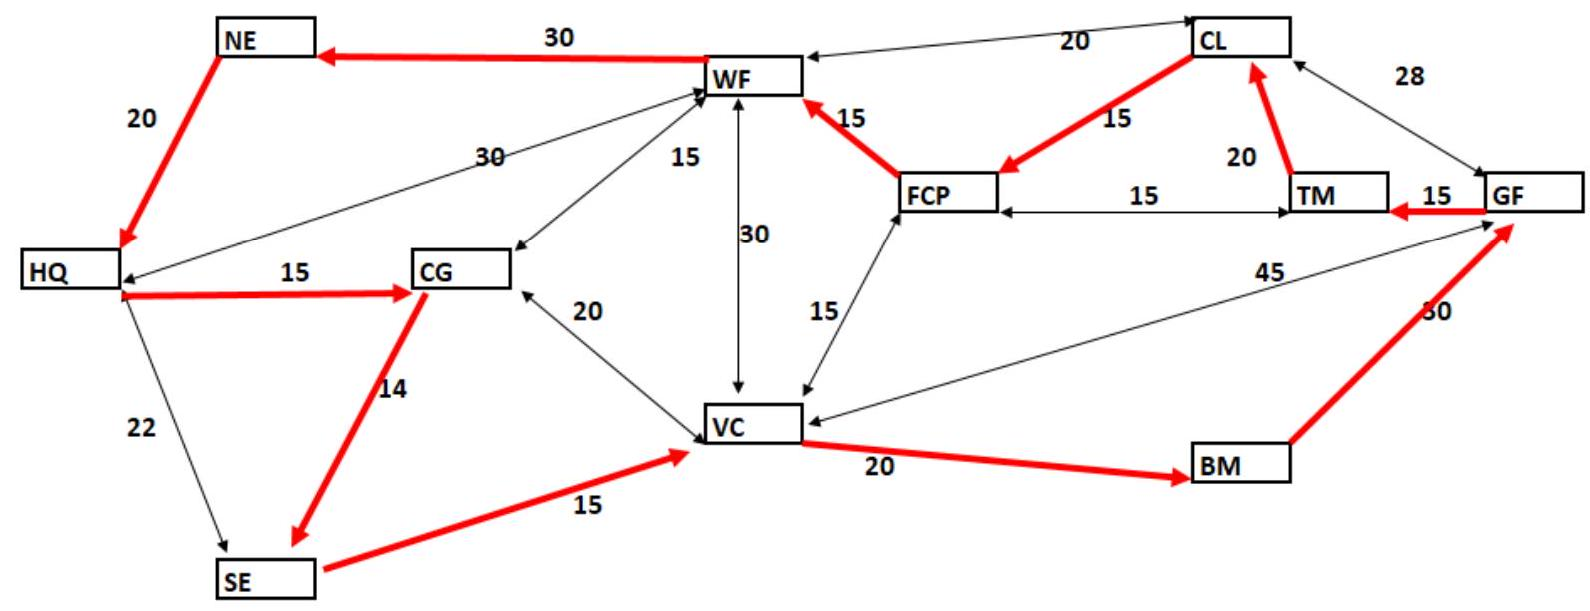
\includegraphics[width=0.5\textwidth]{2024_12_09_1e11ad6a3005a73458cag-18}

\section*{TSP using Excel}
To use Excel to solve the TSP problem, we first have to set up the distance matrix. It shows the distance in minutes between each pair of nodes. As we have done earlier, we set this value to a large number when no such path exists to make sure that option is never chosen. Note that the matrix is symmetrical, this is because all our roads can be driven in either direction. If we had one-way roads the matrix would no longer be symmetrical.

This is no longer a linear programming problem. For example, we assign the different nodes arbitrary numbers, so the contribution of the decision variables to the value of the objective function is no longer proportional to their value. Excel offers two other solver options: A generalized reduced gradient algorithm and an evolutionary algorithm. The details of these algorithms are a bit beyond this class, though I am happy to talk to you outside the class room if you are interested. Basically, the GRG method finds the direction of steepest increase or decrease to move towards the maximum/minimum. It works well if the objective functions and feasible region are smooth-ish (think parabolas, cones, etc.). The evolutionary algorithm does not have any smoothness requirements. It uses a random start point and then evolves the next generation of solution points from that start point (a little like the path-reversal, but with a strong random element). It does not use gradient information, so you cannot be sure you reached the best solution. The evolutionary solver will keep searching for better solutions until it no longer makes sufficient progress or runs out of time. We will use the Evolutionary Solver option.

We start with an arbitrary sequence 1-2-3-4-5-6-7-8-9-10-11-1. The INDEX function is used to look the associated time in the distance matrix.

Syntax: =INDEX(range where to look, what row to use, optional: what column to use)\\
The objective function is simply the sum of the times. As our only constraint we use the "all different" option. The constraint "\$C\$22:\$C\$32 = AllDifferent" means that the 11 decision variables stored in $\$ C \$ 22: \$ C \$ 32$ must be integers in the range 1-11, with each one different from all the others, i.e. we require permutations of $\{1,2,3,4,5,6,7,8,9,10,11\}$. Finally, you want to choose the option to set a time limit for your solver, 60 seconds should be sufficient.\\
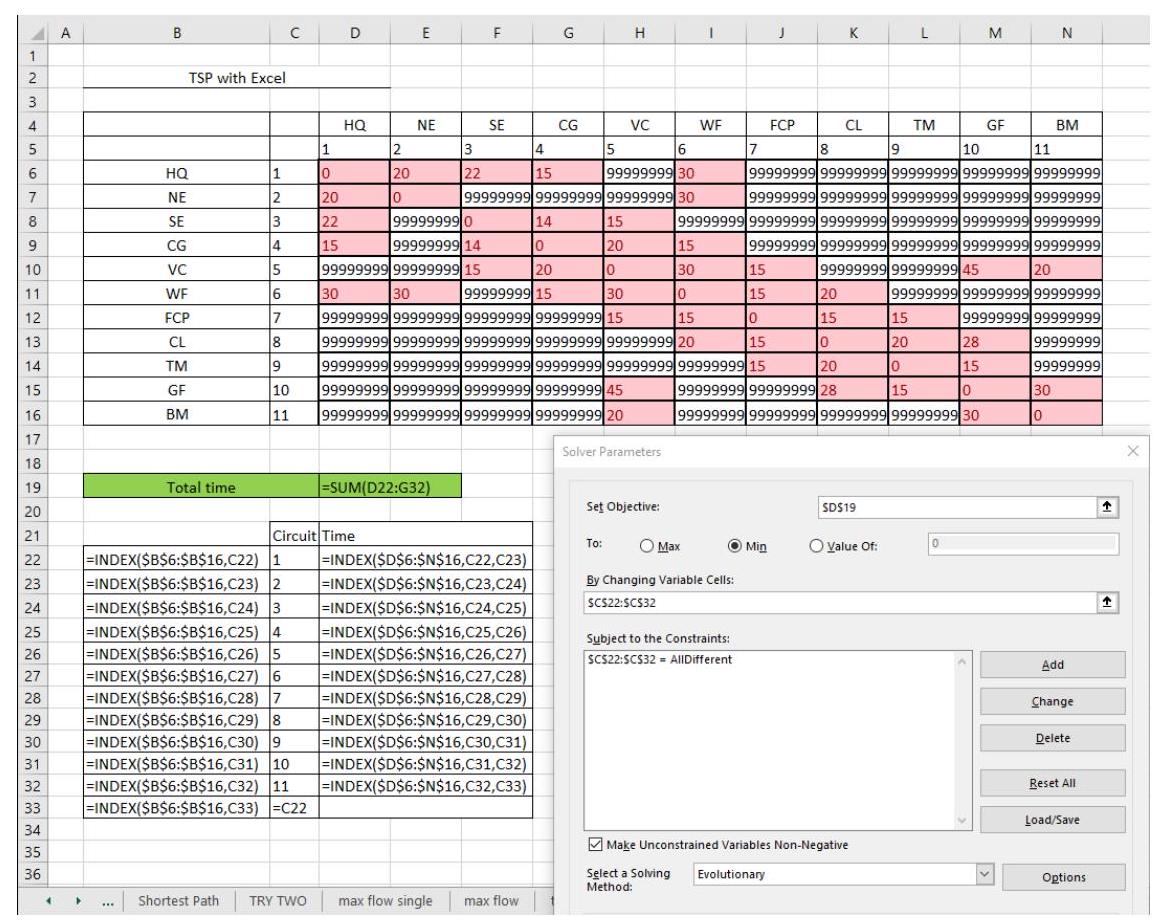
\includegraphics[width=0.5\textwidth]{2024_12_09_1e11ad6a3005a73458cag-19}

The solver returns the solution below. The time requirement is the same as we found in our previous attempts.

\begin{center}
\begin{tabular}{|c|c|l|}
\cline { 2 - 3 }
\multicolumn{1}{c|}{} & Circuit & Time \\
\hline
WF & 6 & 20 \\
\hline
CL & 8 & 15 \\
\hline
FCP & 7 & 15 \\
\hline
TM & 9 & 15 \\
\hline
GF & 10 & 30 \\
\hline
BM & 11 & 20 \\
\hline
VC & 5 & 15 \\
\hline
SE & 3 & 14 \\
\hline
CG & 4 & 15 \\
\hline
HQ & 1 & 20 \\
\hline
NE & 2 & 30 \\
\hline
WF & 6 &  \\
\hline
\end{tabular}
\end{center}

\section*{Stating the Solution}
Starting at HQ, the route traveled will take 209 minutes or 3 hours 29 minutes. An optimal route to take is $\mathrm{HQ} \rightarrow \mathrm{NE} \rightarrow \mathrm{WF} \rightarrow \mathrm{CL} \rightarrow \mathrm{FCP} \rightarrow \mathrm{TM} \rightarrow \mathrm{GF} \rightarrow \mathrm{BM} \rightarrow \mathrm{VC} \rightarrow \mathrm{SE} \rightarrow \mathrm{CG} \rightarrow \mathrm{HQ}$. An alternate of same length is $\mathrm{HQ} \rightarrow \mathrm{NE} \rightarrow \mathrm{WF} \rightarrow \mathrm{FCP} \rightarrow \mathrm{CL} \rightarrow \mathrm{TM} \rightarrow \mathrm{GF} \rightarrow \mathrm{BM} \rightarrow \mathrm{VC} \rightarrow \mathrm{SE} \rightarrow \mathrm{CG} \rightarrow \mathrm{HQ}$, and of course both routes can be reversed.

\section*{Part 5: Road Patrols - Traversing}
To ensure the safety of visitors, a ranger has to patrol the entire road system in the park daily, starting and ending at HQ while minimizing travel time. If possible, they should drive each road only once in either direction. In graph theory, a path that visits each arc in a graph exactly once and ends and starts at the same vertex is called a Eulerian circuit. You may recall from Discrete Mathematics that a Euler circuit exists if and only if the degree of each vertex is even, i.e. an even number of edges connect to each vertex. Unfortunately, that is not the case here, SE and TM both have degree 3.\\
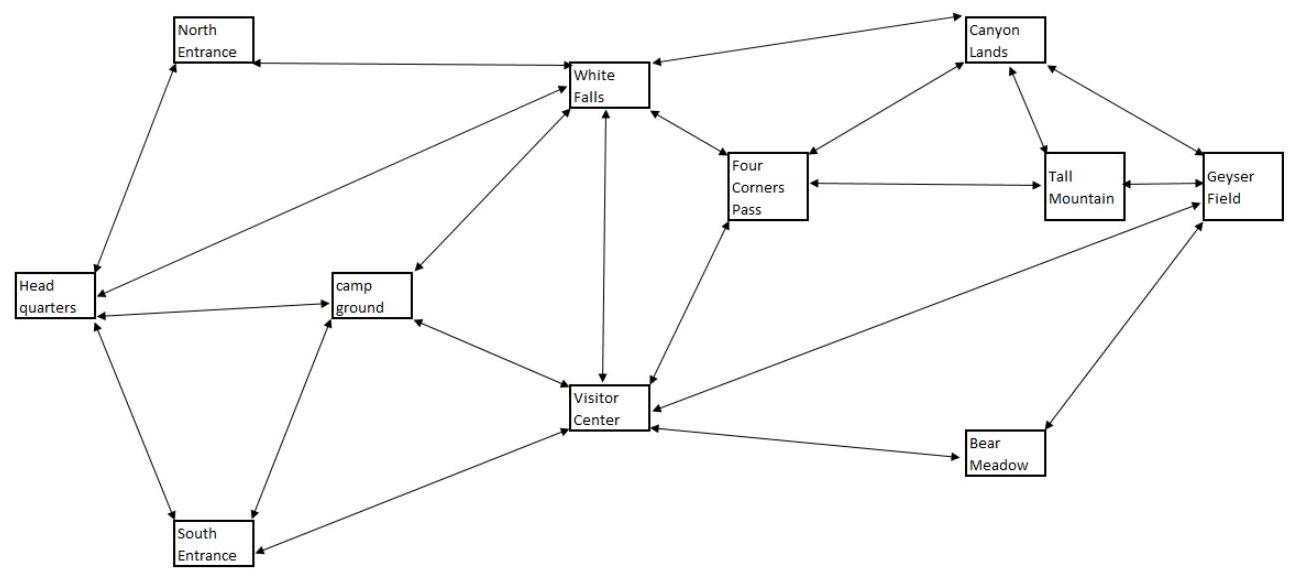
\includegraphics[width=0.5\textwidth]{2024_12_09_1e11ad6a3005a73458cag-20}

We already know that it is not possible to traverse each road exactly once, so the question now becomes how many times each road needs to be traveled, and in which direction. We re-arrange our table to list both road directions next to each other. This makes it easier to write the constraints: "each segment needs to be traveled at least once in either direction".\\
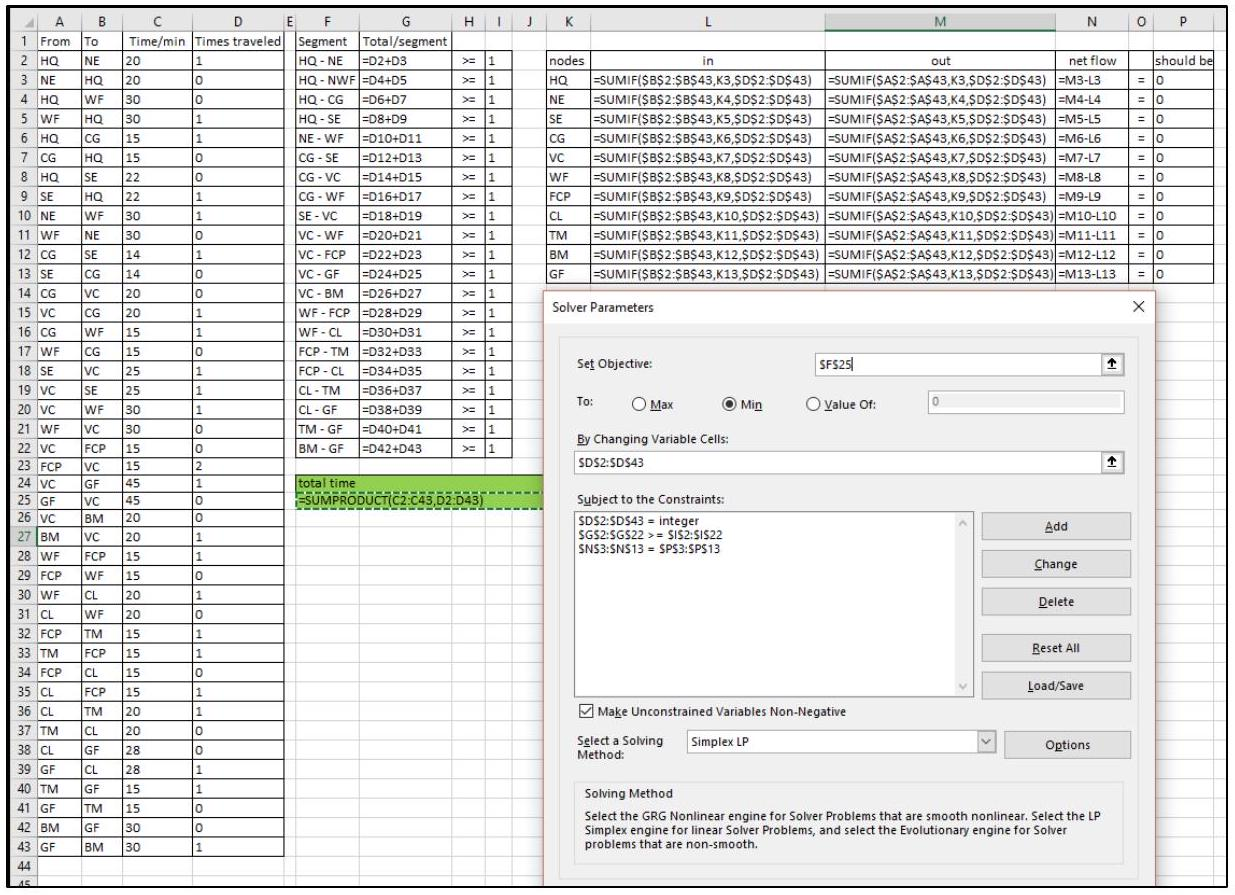
\includegraphics[width=0.5\textwidth]{2024_12_09_1e11ad6a3005a73458cag-20(1)}

\section*{Stating the Solution}
It will take a single ranger 514 minutes or 8 hours 34 minutes to patrol all the roads in the park. One possible optimal route is:\\
$\mathrm{HQ} \rightarrow \mathrm{NE} \rightarrow \mathrm{WF} \rightarrow \mathrm{HQ} \rightarrow \mathrm{CG} \rightarrow \mathrm{WF} \rightarrow \mathrm{FCP} \rightarrow \mathrm{VC} \rightarrow \mathrm{WF} \rightarrow \mathrm{CL} \rightarrow \mathrm{FCP} \rightarrow \mathrm{TM} \rightarrow \mathrm{GF} \rightarrow \mathrm{CL} \rightarrow \mathrm{TM} \rightarrow \mathrm{FCP} \rightarrow \mathrm{VC} \rightarrow \mathrm{GF} \rightarrow \mathrm{BM} \rightarrow \mathrm{VC}$\\
$\rightarrow \mathrm{CG} \rightarrow \mathrm{SE} \rightarrow \mathrm{VC} \rightarrow \mathrm{SE} \rightarrow \mathrm{HQ}$. This is just one of many options. The only rule is that either all roads have to be travelled in the direction and frequencies shown, or all directions have to be reversed.\\
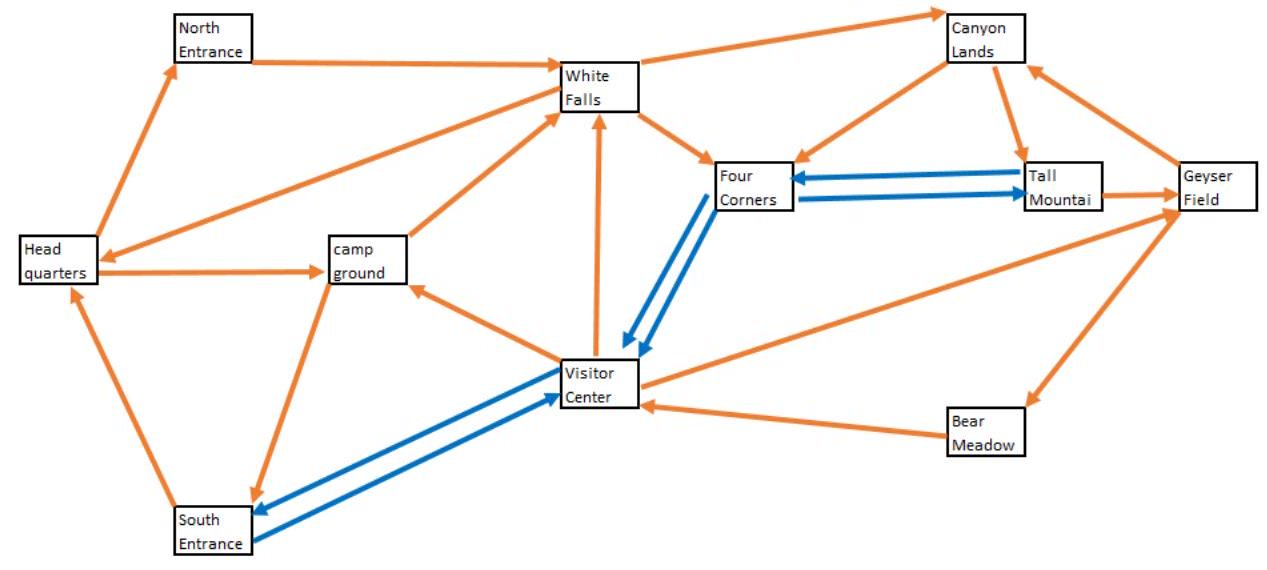
\includegraphics[width=0.5\textwidth]{2024_12_09_1e11ad6a3005a73458cag-21}

The patrol as specified is not possible without overtime, especially not if anything needs attention. Possible alternatives are:

\begin{itemize}
  \item Splitting the area between two or more patrols or two or more days
  \item Eliminating roads from the patrol
  \item Faster car?
\end{itemize}

Comment: Note that this is a Euler path if you eliminate the second traversals. Basically, we have a Euler path from SE to TM + the fastest way / shortest path linking the beginning and end of that Euler path. If you think of each arrow as an undirected arc, then all nodes have even degree and a Euler circuit exists. Basically, we figured out where edges need to be added to have the cheapest possible Euler path/circuit.

%
%\end{document}